\documentclass[12pt,a4paper]{report}

\usepackage[dutch]{babel}
\usepackage{colortbl}

\usepackage{graphicx}
\DeclareGraphicsExtensions{.pdf,.png,.jpg}

\usepackage{textcomp}

\usepackage{eurosym}
\usepackage{hyperref}

\usepackage{caption}
%%\captionsetup[figure]{slc=off} % "slc" is an abbreviation for "singlelinecheck"
\captionsetup{justification=raggedright,singlelinecheck=false}

\usepackage{subcaption}

\usepackage{geometry}
\geometry{a4paper,total={180mm,257mm},left=20mm,top=20mm}

%% Use no serif font for text, courier for commands
\newcommand*{\myfont}{\fontfamily{lmss}\normalsize\selectfont}
\newcommand*{\monofont}{\fontfamily{pcr}\scriptsize\selectfont}

\newcommand*{\marklin}{M\"{a}rklin}
\newcommand*{\trace}{trac\'{e} }
\newcommand*{\isqc}{I$^{2}$C}

\setlength{\parindent}{0pt}

\pagestyle{headings}

\begin{document}

\myfont

\title{
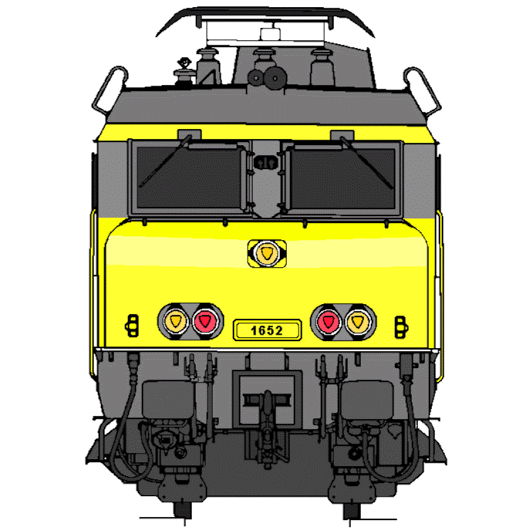
\includegraphics[scale=0.6]{images/RCU_logo}
\makebox[\linewidth]{\rule{\textwidth}{0.4pt}}
Railclub Utrecht
\vfill
Normen H0 groep\\
\makebox[\linewidth]{\rule{\textwidth}{0.4pt}}
\vfill
\small
\author{Peter Mansvelder}
\begin{tabular}{| l | l |}
\hline
\cellcolor[gray]{0.84}Titel & Normen H0 groep Railclub Utrecht\\
\hline
\cellcolor[gray]{0.84}Auteur & Peter Mansvelder\\
\hline
\cellcolor[gray]{0.84}Eigenaar & Marc Timmermans / Peter Mansvelder\\
\hline
\cellcolor[gray]{0.84}Versie & 3 (concept)\\
\hline
\cellcolor[gray]{0.84}Versiedatum & \today\\
\hline
\cellcolor[gray]{0.84}Status & Concept\\
\hline
\end{tabular}
}

\maketitle

\tableofcontents

\listoffigures

\listoftables

\chapter{Opbouw document}

\section{Documentoverzicht}

Hoofdstuk 1 geeft de opbouw en overzicht van dit document.

Hoofdstuk \ref{ch:normen} geeft een korte inleiding tot het systeem en de normen.

Hoofdstuk \ref{ch:modules} beschrijft de mechanische opbouw van de modules.

Hoofdstuk \ref{ch:rails} beschrijft het leggen van de rails.

Hoofdstuk \ref{ch:elektra} beschrijft de normen van de elektrische installatie.

Hoofdstuk \ref{ch:beveiliging} beschrijft de beveiling van de baan.

Hoofdstuk \ref{ch:bovenleiding} beschrijft de bovenleiding.

Hoofdstuk \ref{ch:landschap} beschrijft de opbouw van het landschap.

Hoofdstuk \ref{ch:electronica} beschrijft de aansluiting van de modules en de booster.

Hoofdstuk \ref{ch:centrale} beschrijft de gebruikte digitale centrale.

\section{Afkortingen en begrippen}

\begin{table}[!ht]
\begin{tabular}{| l |p{13cm}|}
\hline
\rowcolor[gray]{0.84}Afkorting & Omschrijving\\
\hline
DCC & Digital Control Systeem, het NMRA-standaard digitale systeem voor modeltreinen.\\
\hline
MM & Motorola, het door \marklin gebruikte digitale systeem\\
\hline
MDRRC-II&Model Digital RailRoad Control, een door Robert Evers gemaakte centrale die zowel DCC als Motorola protocol ondersteunt. Versie II is gebaseerd op een microcontroller met touchscreen.\\
\hline
RCU&RailClub Utrecht.\\
\hline
BNL&Beneluxspoor, een forum voor Nederlands Modelspoorders.\\
\hline
S88&Een door \marklin \ ge"{i}ntroduceerde standaard voor bezetmelders (eigenlijk massamelders).\\
\hline
\isqc &Inter-Integrated Circuit, een door Philips ge"{i}ntroduceerde computer bus voor seri"{e}le communicatie.\\
\hline
XpressNet&Ook Roconet of XBus genoemd, door Lenz ge"{i}ntroduceerde bus voor communicatie van digitale modelspoorcomponenten.\\
\hline
\end{tabular}
\caption{Gebruikte afkortingen}
\end{table}

\chapter{Inleiding}
\label{ch:normen}
M-track is een modulair systeem voor half nul met een middenrail, waarbij de beide spoorstaven elektrisch gescheiden zijn. Bij de RailClub Utrecht wordt dit systeem gebruikt om zowel 2- als 3-rail systeem rollend materieel te laten rijden.

Dit document beschrijft de norm voor M-track, die we bij Railclub Utrecht gebruiken. Voor zaken die niet in de norm geregeld zijn is het zinvol die eerst met de moduleco\"{o}rdinator te overleggen.

Voor de leden die besluiten mee te doen met deze modulebaan is het raadzaam eerst te kijken hoe dingen in elkaar steken en te vragen als er iets niet duidelijk is.

\section{Systeemnormen}
De systeemnormen van M-track bestaan uit:
\begin{itemize}
\item Het gebruikte (digitale) systeem
\item Een genormaliseerde kopkant van de modules;
\item Een minimum boogstraal van de hoofdbaan;
\item Het type wissels dat gebruikt kan worden in de hoofdbaan;
\item De hoogte van de sporen t.o.v. de vloer.
\end{itemize}

De afspraken zijn als volgt:

\begin{table}[!ht]
\begin{tabular}{| l |p{7cm}|}
\hline
\cellcolor[gray]{0.84}Digitaal Systeem & Gecombineerd DCC/Motorola\\
\hline
\cellcolor[gray]{0.84}Lengte standaard module & Aanbeveling max. 1200 mm\\
\hline
\cellcolor[gray]{0.84}Breedte standaardmodule & 600 mm\\
\hline
\cellcolor[gray]{0.84}Hoogte standaardmodule & Voorzijde 120 mm, Spoordijk 150 mm hoog\\
\hline
\cellcolor[gray]{0.84}Hoogte bovenkant spoorstaaf t.o.v. de vloer&1200 mm $\pm$ 25 mm\\
\hline
\cellcolor[gray]{0.84}Aantal sporen&Twee\\
\hline
\cellcolor[gray]{0.84}Hartafstand van de sporen K-Rail 2200 serie&57 mm\\
\hline
\cellcolor[gray]{0.84}Minimum boogstraal binnenboog&Grote cirkel 1 van \marklin, radius 553,9 mm\\
\hline
\cellcolor[gray]{0.84}Minimum boogstraal buitenboog&Grote cirkel 2 van \marklin, radius 618,5 mm\\
\hline
\cellcolor[gray]{0.84}Type wissels&2272, 2273, 2275, 22715 en 22716\\
\hline
\cellcolor[gray]{0.84}Materiaal voor de constructie van de modulen&Multiplex 12 mm\\
\hline
\cellcolor[gray]{0.84}Constructie&Open raambouw methode\\
\hline
\cellcolor[gray]{0.84}Afstand tussenschotten&Maximaal 400 mm\\
\hline
\cellcolor[gray]{0.84}Kleur voorzijde&Schoolbordenverf, zwart\\
\hline
\cellcolor[gray]{0.84}Poten&Volgens tekening, in hoogte te verstellen tot $\pm$ 25 mm\\
\hline
\cellcolor[gray]{0.84}De bovenleiding&Sommerfeldt\\
\hline
\end{tabular}
\caption{Normen en afspraken}
\end{table}

\chapter{Modules}
\label{ch:modules}
Het systeem is opgebouwd uit modules. Er zijn verschillende modules mogelijk:

\section{Maten kopschotten}

Dit zijn de gebruikte profielen van de kopschotten, de voorkant van de module is steeds links:

\begin{figure}[!ht]
  \captionbox
  {Open Module, symmetrisch}
  {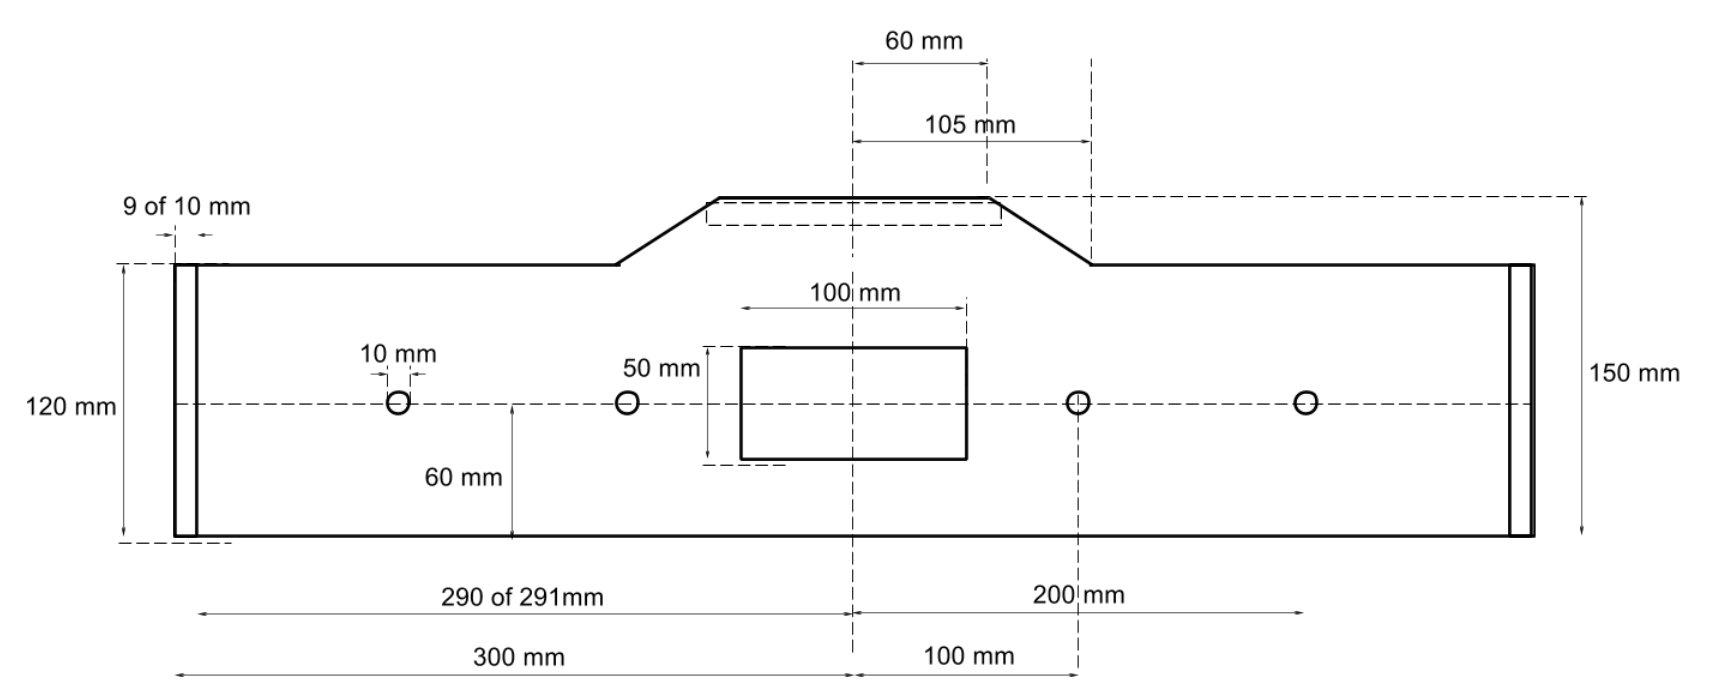
\includegraphics[scale=0.25]{images/rcu_open_sym}}
\end{figure}

\begin{figure}[!ht]
  \captionbox
  {Open Module, asymmetrisch}
  {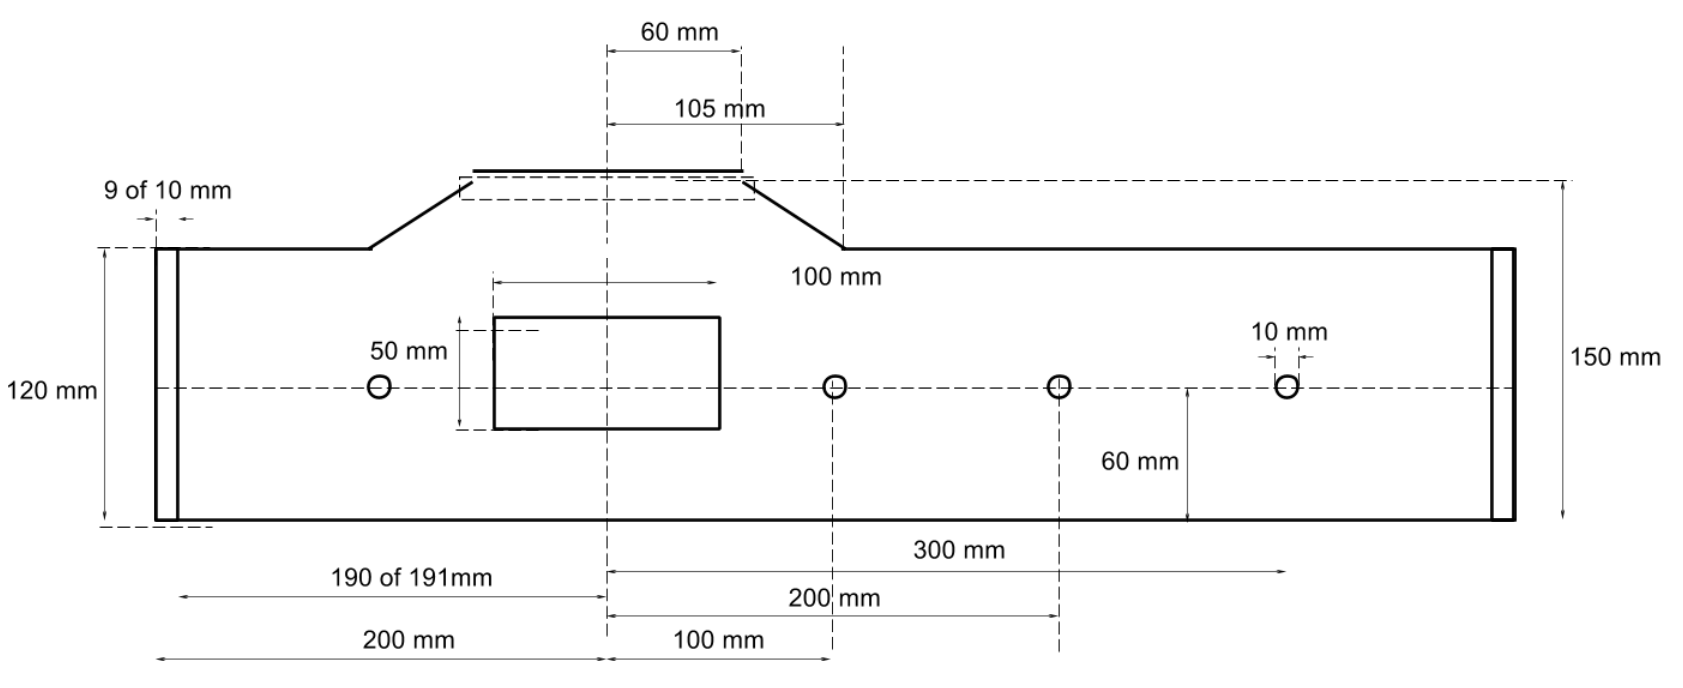
\includegraphics[scale=0.25]{images/rcu_open_asym}}
\end{figure}

\begin{figure}[!ht]
  \captionbox
  {Vlakke Module, symmetrisch}
  {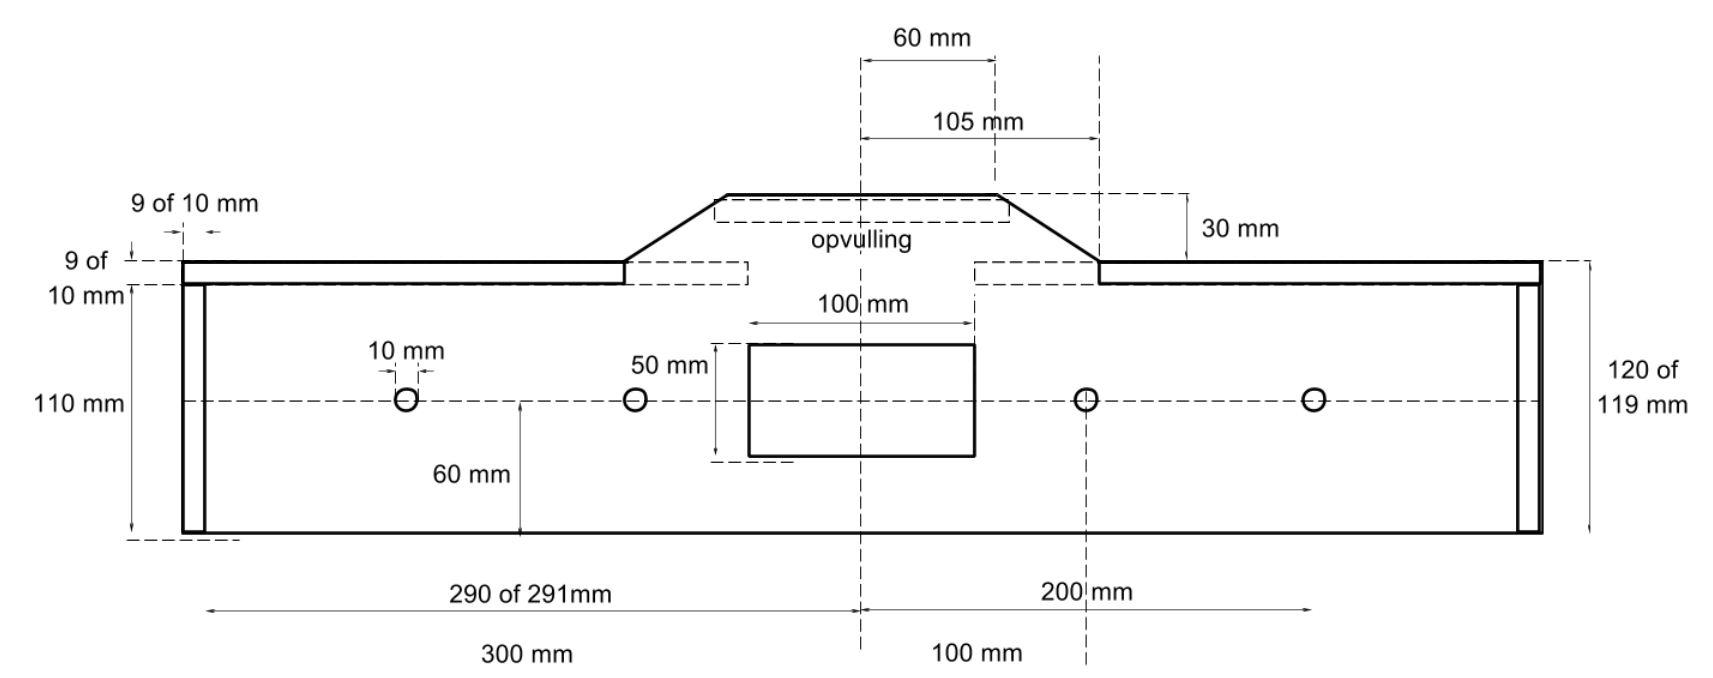
\includegraphics[scale=0.25]{images/rcu_vlak_sym}}
\end{figure}

\begin{figure}[!ht]
  \captionbox
  {Vlakke Module, asymmetrisch}
  {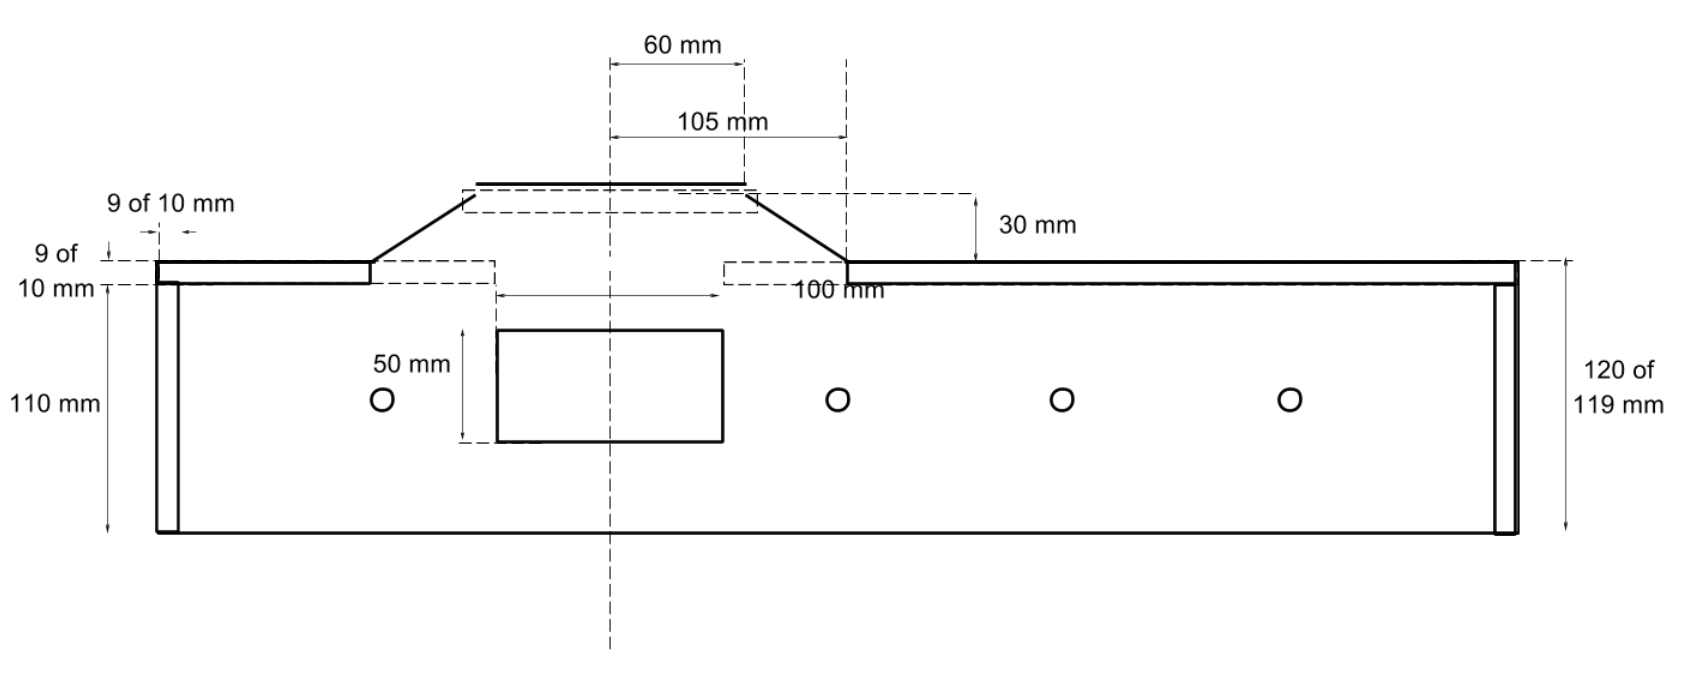
\includegraphics[scale=0.25]{images/rcu_vlak_asym}}
\end{figure}

\begin{figure}[!ht]
  \captionbox
  {Jeugdmodule, asymmetrisch\label{im:jeugdbak}}
  {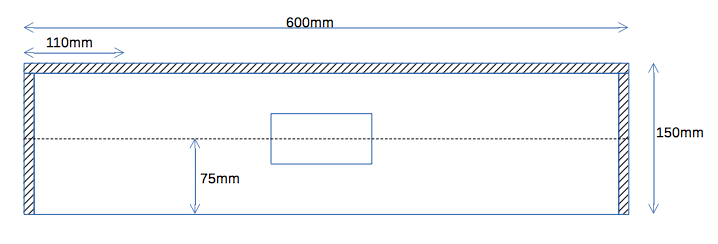
\includegraphics[scale=0.9]{images/jeugdbak}}
\end{figure}

\section{De rechte module met spoordijk}
De rechte module voor de vrije baan, deze kan een lengte hebben van 580 mm, 890 mm of de ''standaard'' lengte van 1200 mm.
Andere lengtematen zijn toegestaan, alleen moet dan rekening gehouden worden met de rijdraadlengte die gebruikt wordt. De rijdraad bij de overgang van de modulen is 270mm lang en op de modulen 310mm.
Bij een standaardmodule is die 3 keer 310mm + 270mm geeft samen de 1200mm lengte.

Een standaard module met spoordijk bestaat uit twee hoofdbestanddelen:
\begin{itemize}
\item De bovenbouw die ook wel de bak wordt genoemd.
\item Vier afneembare poten, deze dienen in hoogte verstelbaar te zijn.
\end{itemize}
Meer info voor de constructie van deze poten, vindt u onder het kopje ''opbouw van de poten'' (paragraaf \ref{se:poten}).

De bovenbouw van de module wordt samengesteld uit twee gelijke kopschotten en twee zijkanten van 120 mm hoog en 1200 mm lang. Daar tussen komen nog twee tussenschotten.
Tussen de kopschotten wordt de ondergrond voor de baan (het \trace) aangebracht. Het \trace rust op de tussenschotten. 

\begin{figure}[!ht]
  \captionbox
  {Opbouw open module\label{figuur1}}
  {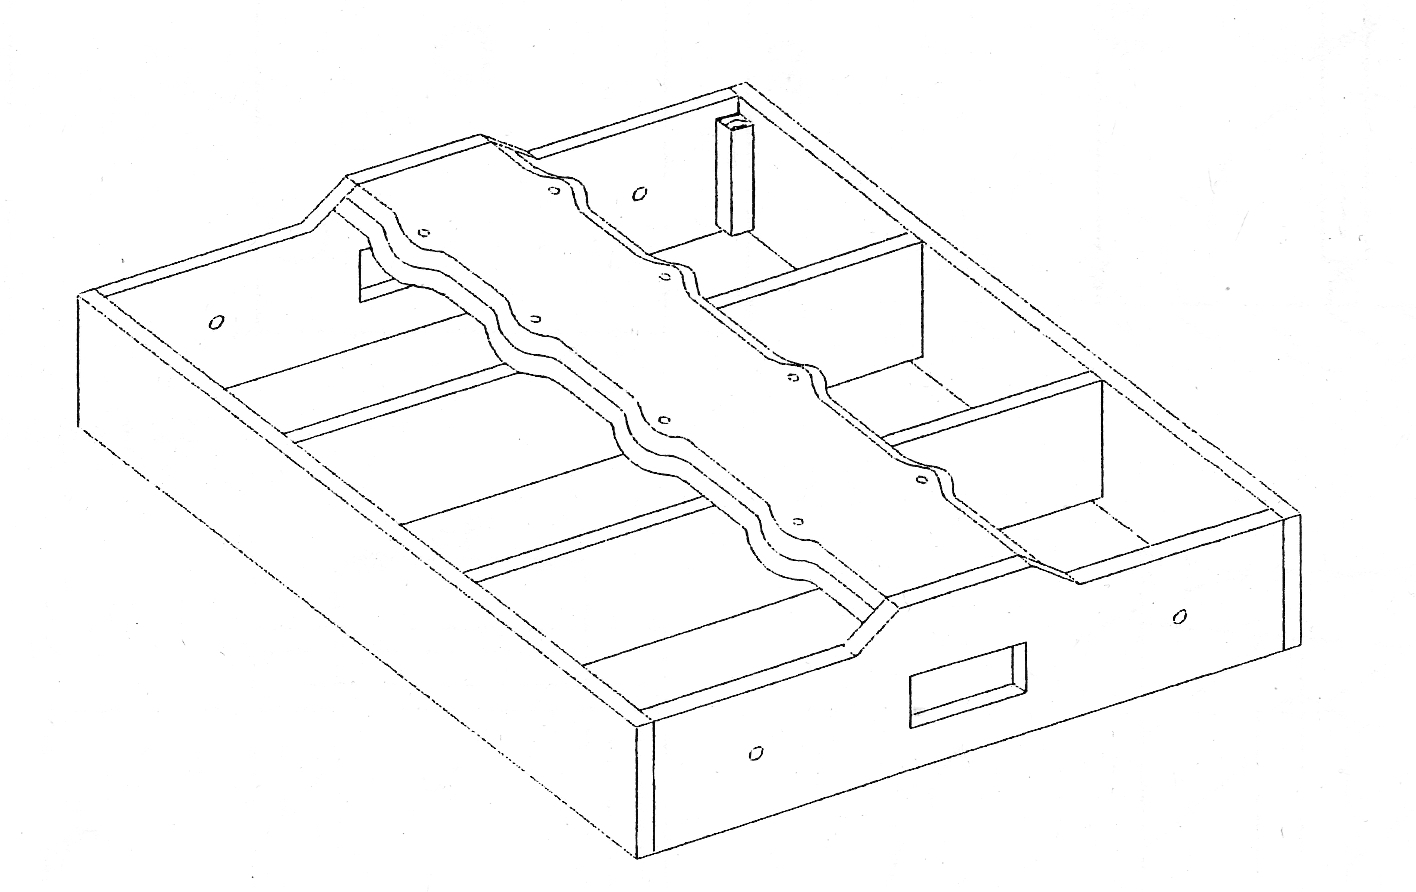
\includegraphics[scale=0.5]{images/rcu_figuur1}}
\end{figure}

Nu trekken we eerst een hartlijn, in het midden van het spoor\trace, van het ene kopschot naar het andere. Dit moet nauwkeurig worden gedaan, omdat vanuit deze lijn de plaats wordt bepaald waar de rails komen te liggen.
Het leggen van de rails wordt behandeld in hoofdstuk \ref{ch:rails}.

Nu worden de gaten geboord waar later de masten voor de bovenleiding in geplaatst worden. 
Hierna kan de moer die onderaan de mast zit ''vast'' worden gedraaid.

\section{De rechte module zonder spoordijk}
Een module zonder spoordijk, met 2 sporen die aan een kant van de module worden gelegd, zodat er meer ruimte is voor scenery aan de achterkant. Dit zijn de oude jeugdmodules (zie figuur \ref{im:jeugdbak} voor profiel).
De hartmaat van de rails is hierbij hetzelfde als de andere modules: 57mm. De rails wordt dicht tegen de voorkant va de bak aangelegd, waarbij de afstand tussen de voorkant van de module en de 1e rail 100mm bedraagt.

\section{Overgangsmodules}
Overgangsmodules tussen de twee verschillende soorten modules (met en zonder spoordijk). Dit kunnen dus verschillende overgangen zijn:
\begin{itemize}
\item Jeugdbak naar symmetrische spoordijk
\item Jeugdbak naar asymmetrische spoordijk
\item Symmetrische spoordijk naar asymmetrische spoordijk
\end{itemize}

\section{De hoekmodule}
De standaard hoekmodule heeft een hoek van $45$\textdegree. Eventueel is een andere hoek ook mogelijk.
Zowel bij de rechte als bij de hoek module is het kopschot uitgevoerd volgens het standaard profiel, zie hiervoor de tekeningen!

Het maken van een standaard hoekmodule is lastiger dan van een rechte module. Een hoekmodule hoeft niet de standaard vorm of hoek te hebben, maar wel het standaard kopschot.

Bij de beschrijving hierna wordt uitgegaan van een standaard hoekmodule. Deze module heeft een hoek van $45$\textdegree. De grootste lengte van de bak is 875 mm en de kleinste lengte 415 mm. De kopzijde is gelijk aan de standaard kopschotten.
De hoek tussen een kopschot en een zijschot is 22,50. Er zijn twee mogelijkheden om dit te realiseren. Men zaagt een balkje onder een hoek of stukjes multiplex. Zie figuur \ref{figuur4}.

\begin{figure}[!ht]
  \captionbox
  {Constructie hoekmodule\label{figuur4}}
  {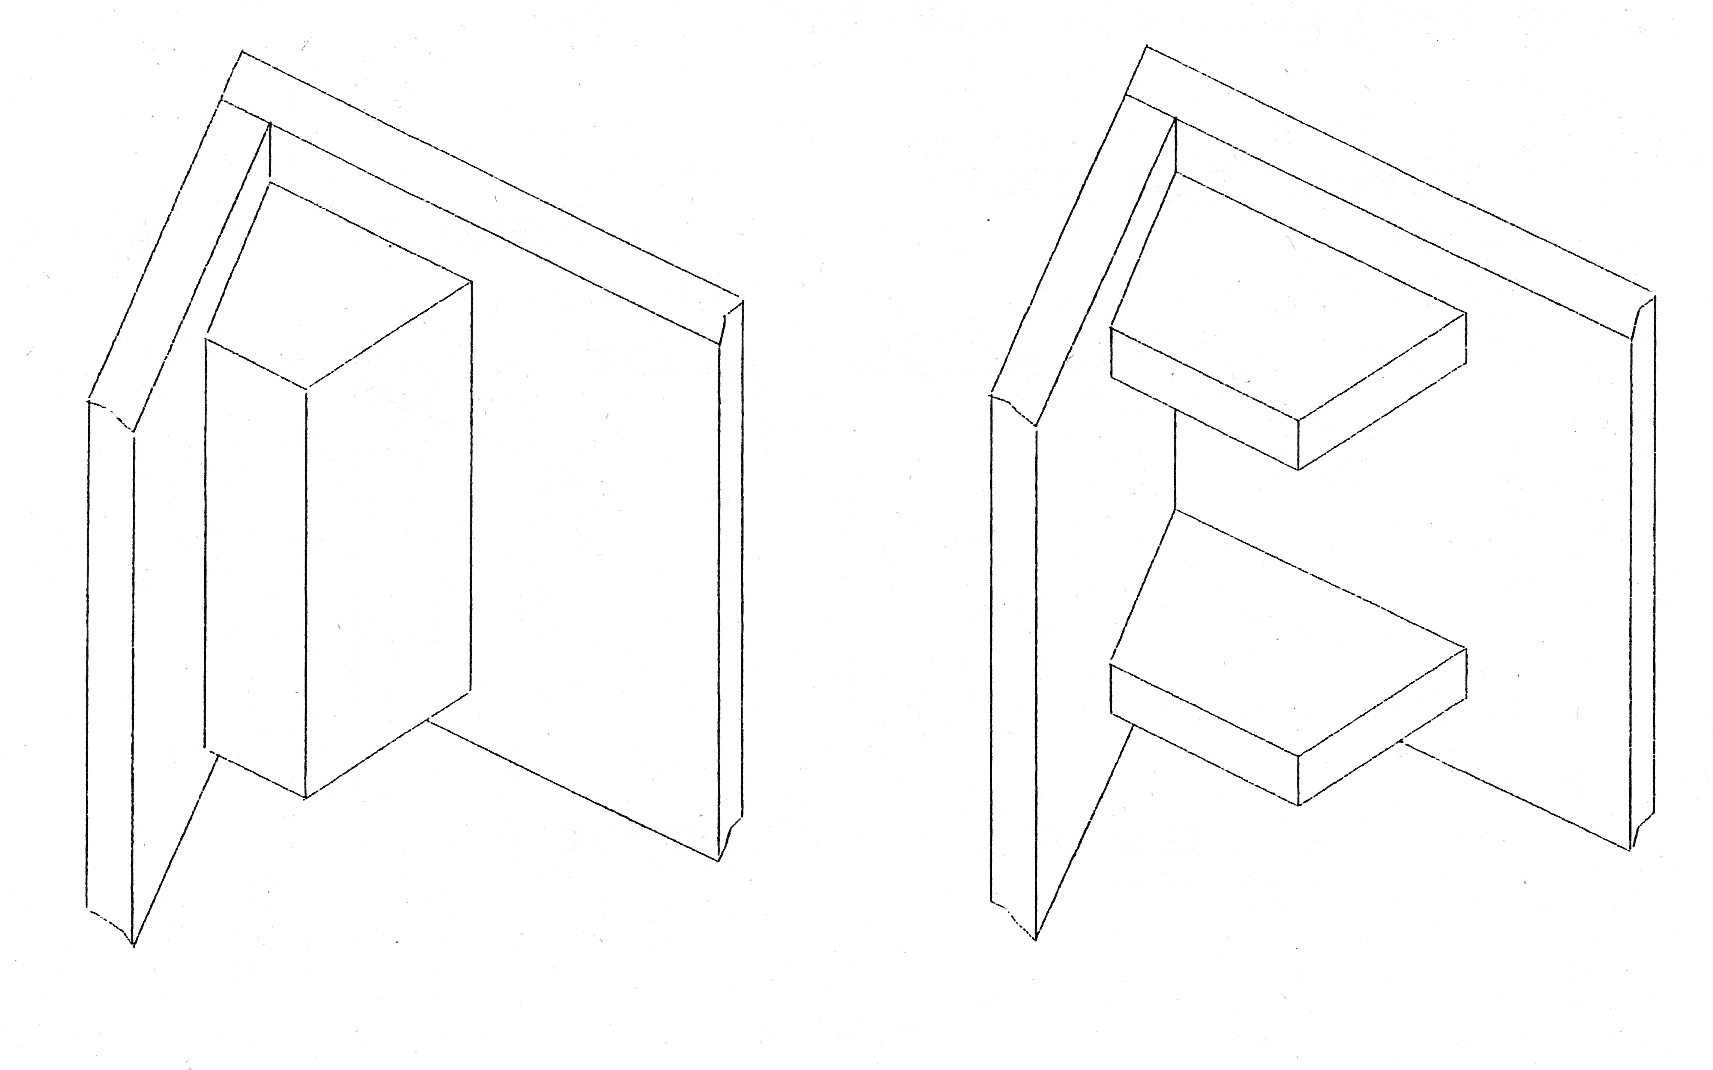
\includegraphics[scale=0.2]{images/rcu_figuur4}}
\end{figure}

Tegen deze hoekversteviging kan dan de standaard constructie voor de poten bevestigd worden. Hierna wordt de ondergrond van het baan\trace bevestigd. Er dient rekening mee gehouden te worden dat de eerste tien centimeter van de rails haaks, t.o.v. het kopschot ligt, en daarna pas de bocht begint. 

Hierna wordt de rails gelegd. Nu worden de gaten geboord waar later de masten voor de bovenleiding in geplaatst worden. 
Hierna kan de moer die onderaan de mast zit ''vast'' worden gedraaid.

\section{De stationsmodules}
Deze bestaan meestal uit meerdere modulen, die altijd op dezelfde wijze aan elkaar gekoppeld worden. Hierdoor hoeft alleen het eerste en het laatste kopschot het standaard profiel te hebben. De tussenliggende kopschotten zijn voor wat betreft de vorm afhankelijk van het sporenplan.

De modules worden opgebouwd van 12 mm dik multiplex. Het beste is om ocum\'{e} triplex te gebruiken. De rails wordt ondersteund door een strook van 8 mm dik multiplex met daarop een 10 mm dikke laag zachtboard of een ander geluiddempend materiaal.
De rest van de module wordt opgebouwd volgens de open raam bouwmethode.

\section{Opbouw poten}
\label{se:poten}
De poten voor de baan zijn allemaal op dezelfde wijze opgebouwd en kunnen zonder problemen met elkaar verwisseld worden. In de bakken zit een standaard constructie waarin de poten geschoven kunnen worden en vastgezet, zie figuur \ref{figuur2}.

\begin{figure}[!ht]
  \captionbox
  {Constructie poten\label{figuur2}}
  {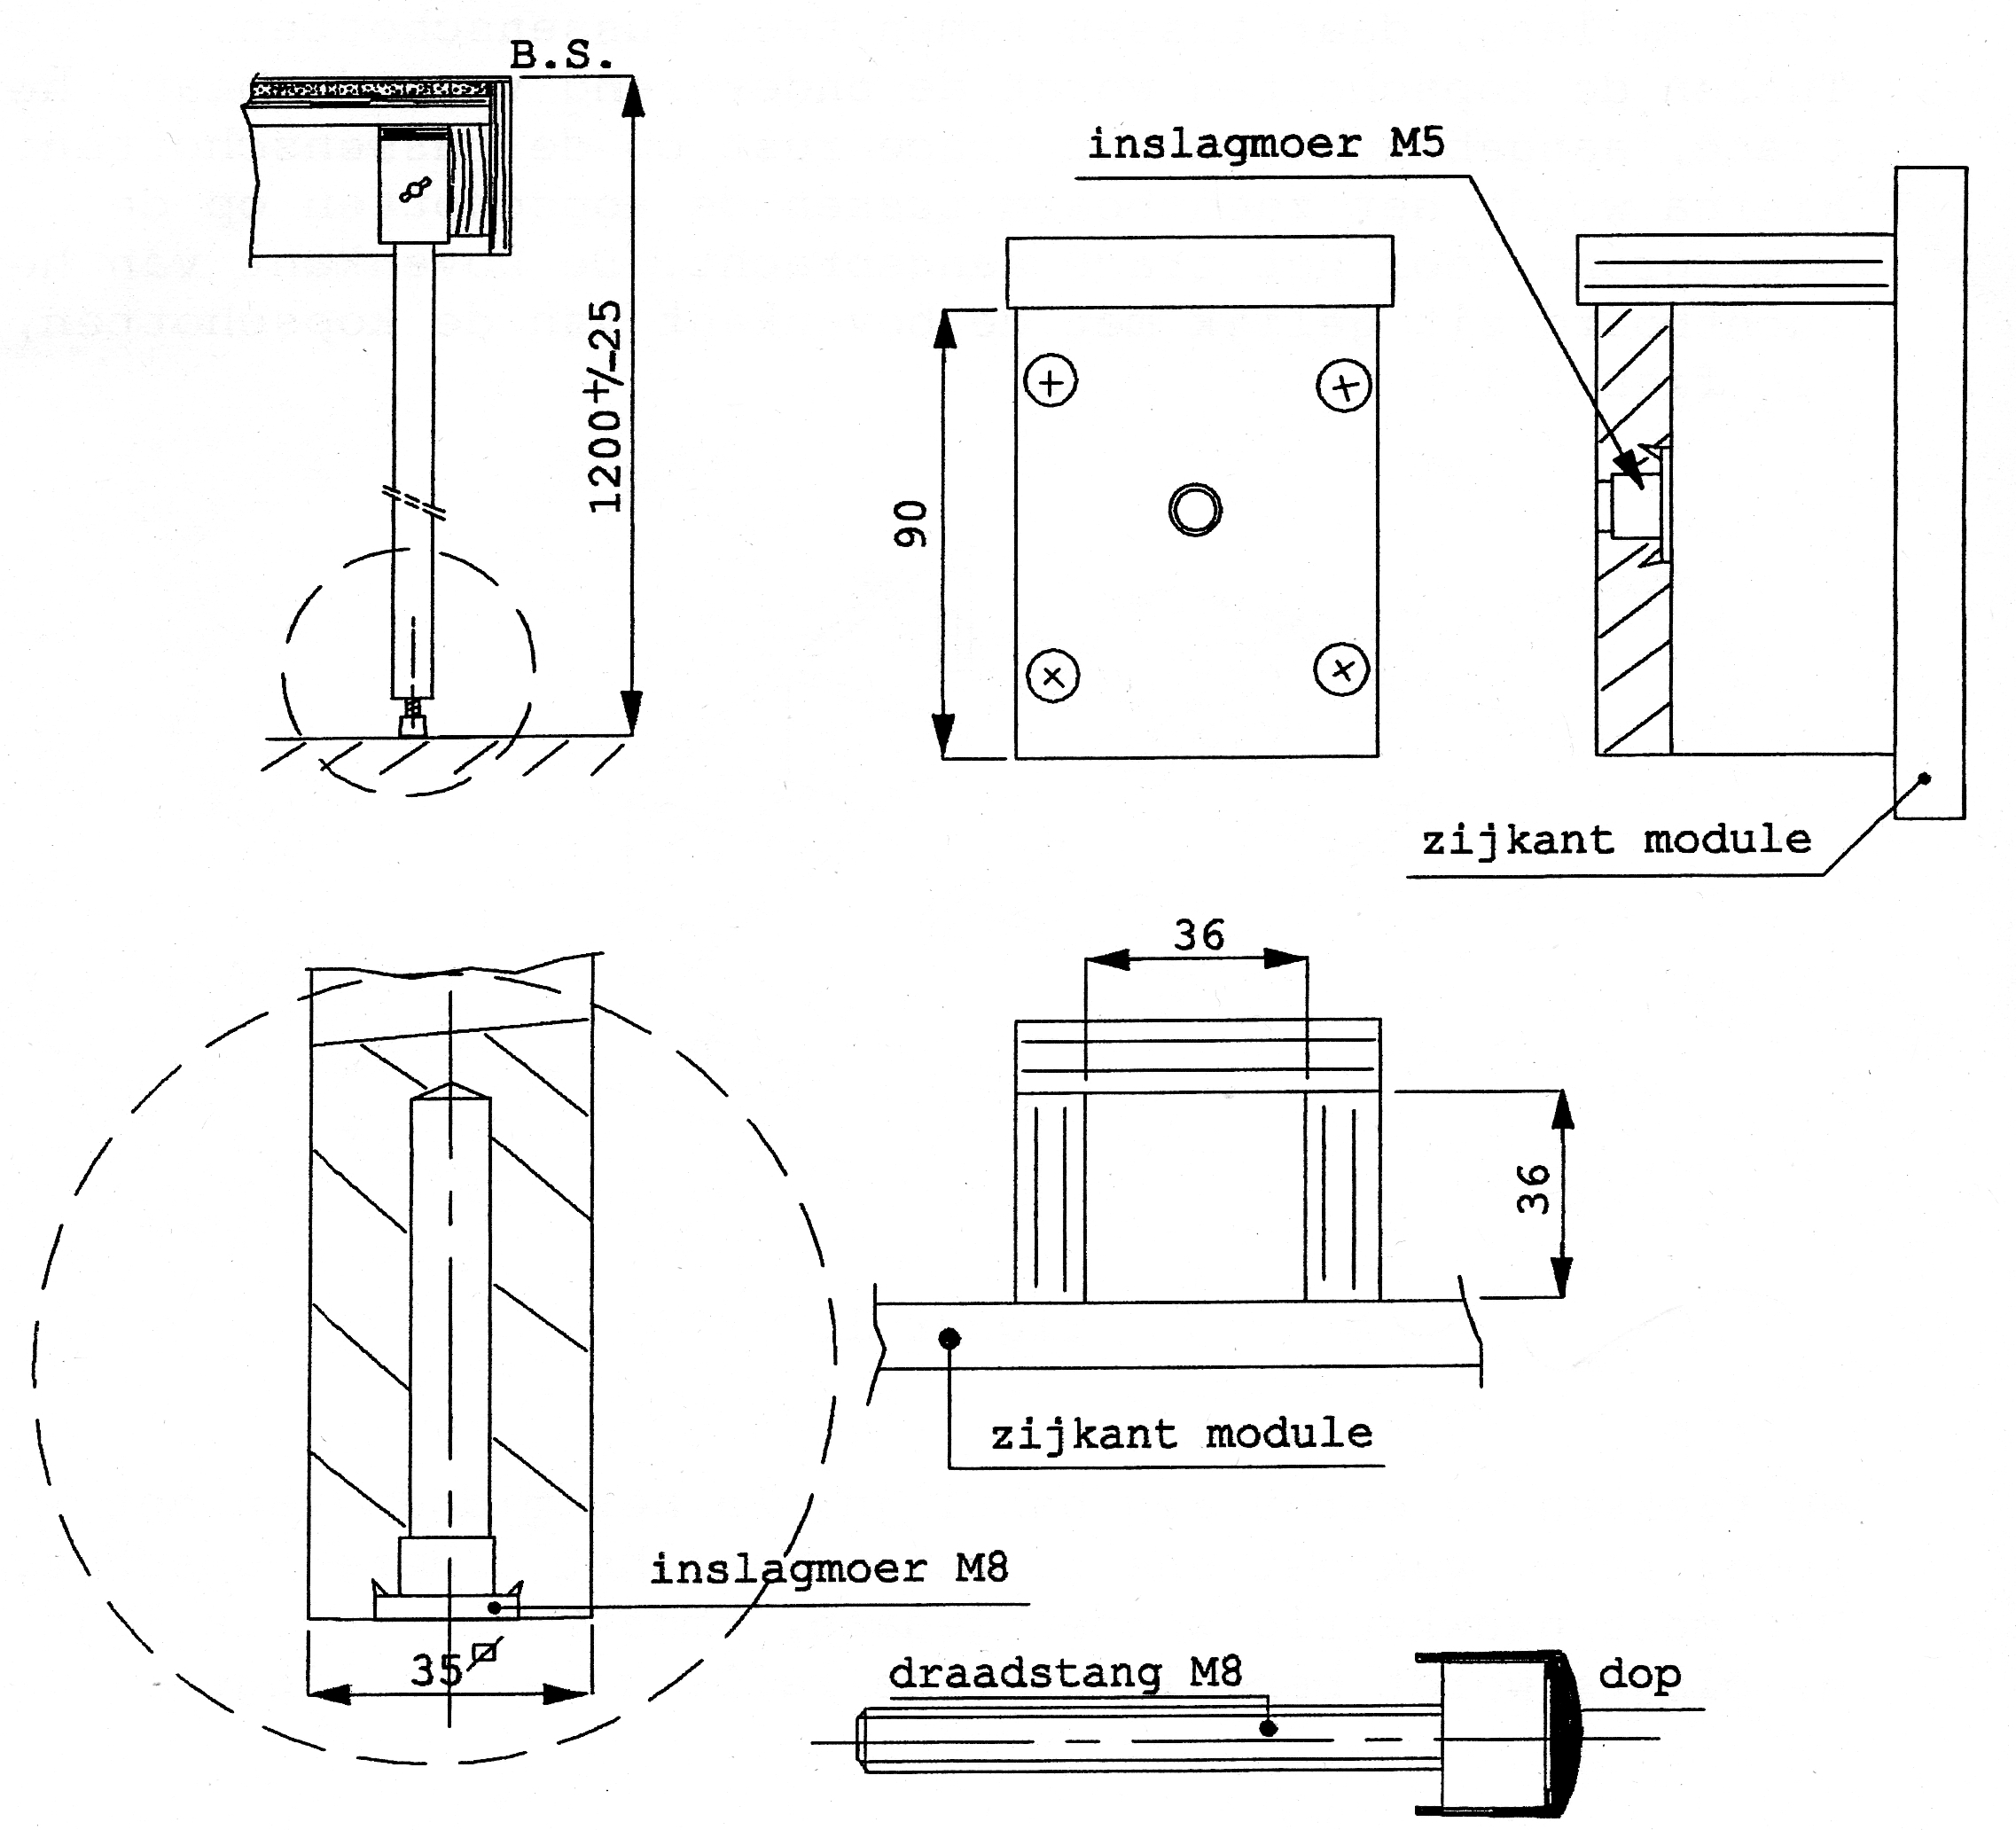
\includegraphics[scale=0.2]{images/rcu_figuur2}}
\end{figure}

De poten kunnen zowel van hout als metaal gemaakt worden en zijn vierkant De poot heeft een dikte van 35 mm en de schacht waarin hij schuift 36 mm. Hierdoor kan de poot altijd makkelijk in en uit genomen worden. Om te voorkomen dat de poot er op het verkeerde moment uitschuift wordt deze met een vleugelboutje vastgezet. Om te voorkomen dat dit vleugelboutje steeds dieper het hout wordt ingedraaid wordt op die plaats een metalen plaatje aangebracht. Zie figuur \ref{figuur3}.

\begin{figure}[!ht]
  \captionbox
  {Bovenzijde poten\label{figuur3}}
  {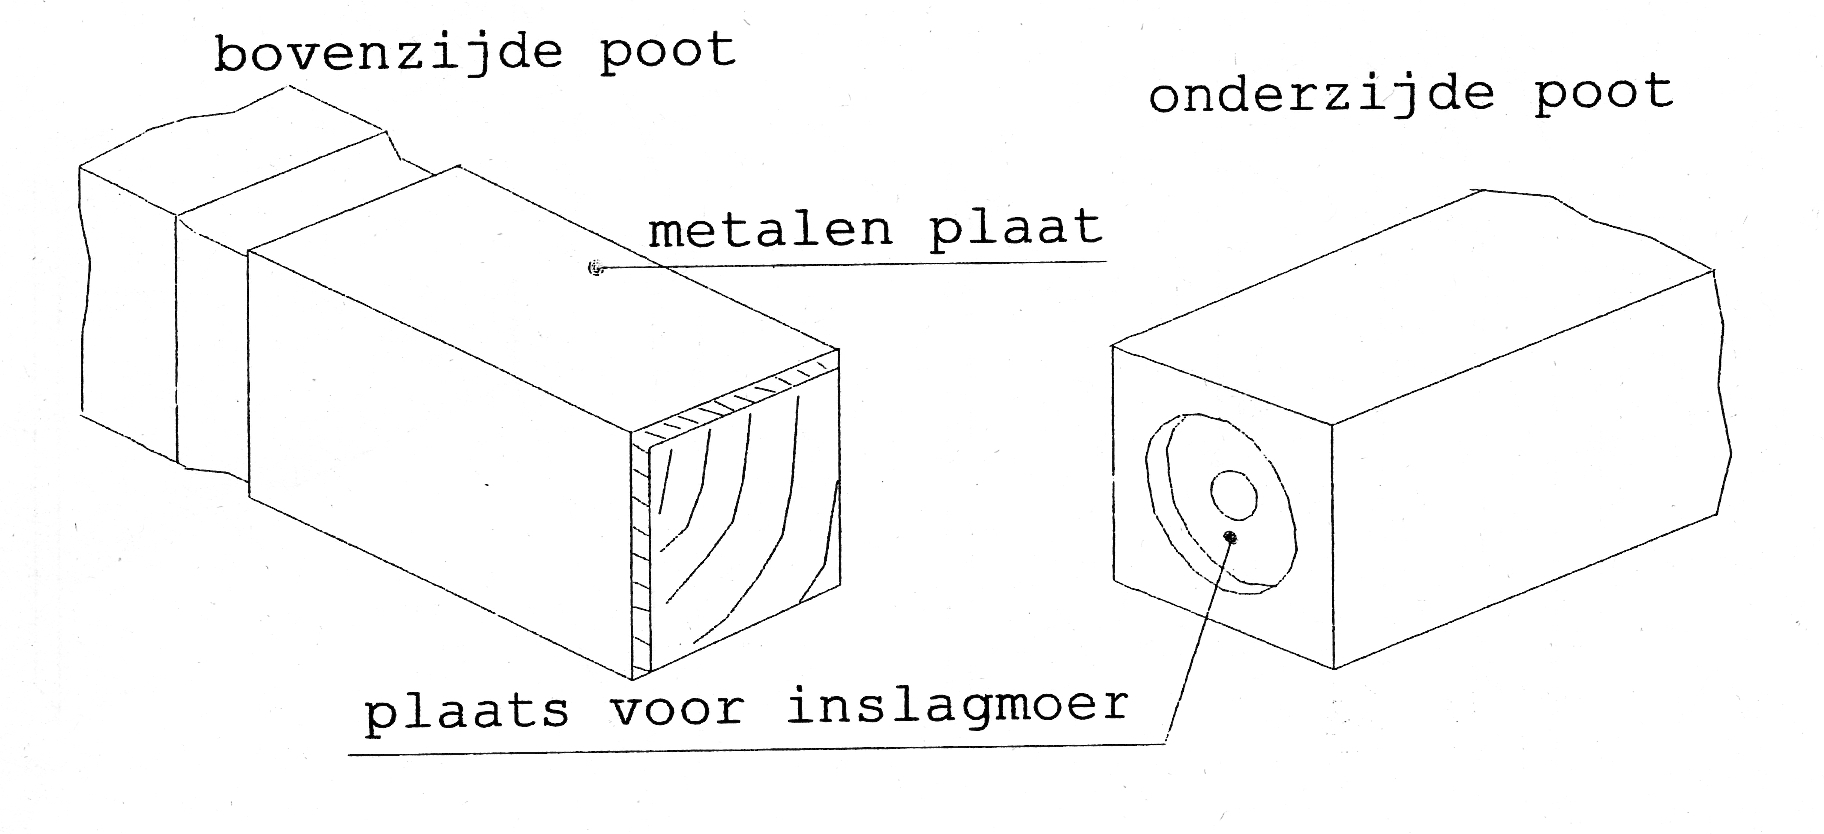
\includegraphics[scale=0.2]{images/rcu_figuur3}}
\end{figure}

De draadstang met daarop een metalen schijf,  met een kunststof dop er overheen, moet voldoende lang zijn om een hoogteverstelling van 50 mm mogelijk te maken.

\section{Achterwanden}
\label{se:achterwanden}
Bij elke module hoort een achterwand, deze is vast bevestigd aan de module. De hoogte van de achterwand is 48 cm (gemeten vanaf bovenkant rails). De achterwand wordt standaard blauw geschilderd (RAL kleur xxx).

\section{Verlichting}
\label{se:verlichting}
Boven elke module komt verlichting in de vorm van een LEDstrip van 100cm per module, uitwisselbaar met andere banen van de RCU. De verlichting is opgebouwd uit de volgende onderdelen:
\begin{itemize}
\item Wandrail 75cm (150 cm in twee stuks gezaagd), gemonteerd aan de achterkant van de achterwanden.
{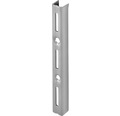
\includegraphics[scale=1.0]{images/wandrail}}
\item Plankdrager 30cm\\
{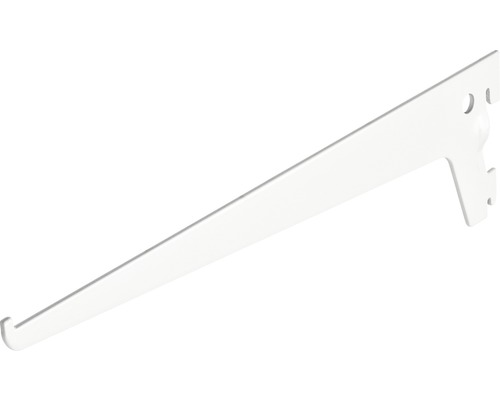
\includegraphics[scale=0.2]{images/plankdrager}}
\item Hoekprofiel kunststof 50x50mm, gezaagd in stukken van 100cm.\\
{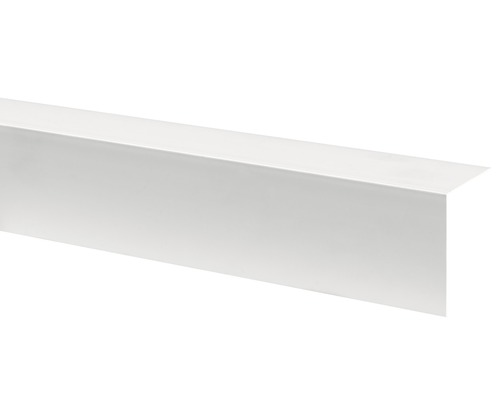
\includegraphics[scale=0.2]{images/hoekprofiel}}
\item LEDstrip 12 volt, 14,4W/m Warmwit, opgedeeld in stukken van 100cm.\\
{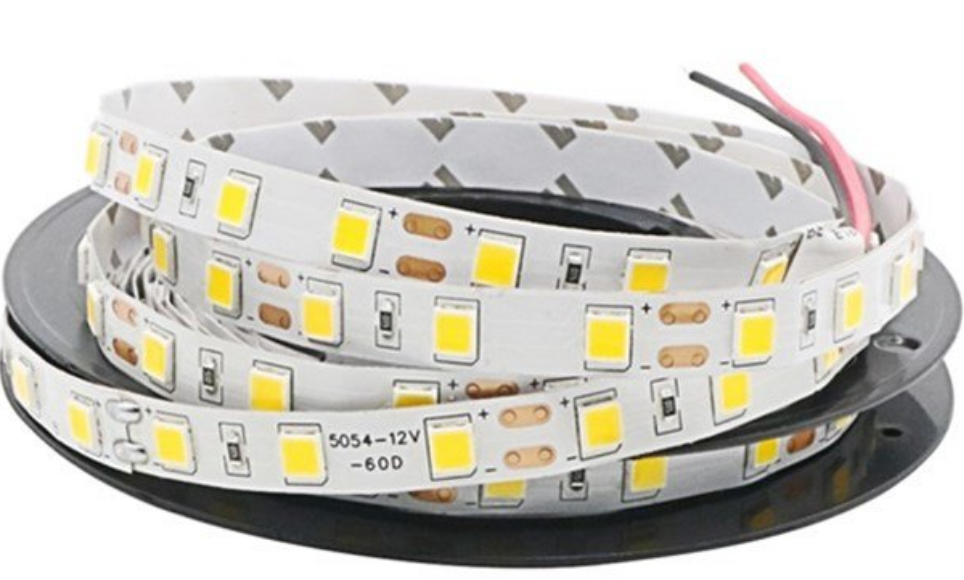
\includegraphics[scale=0.2]{images/ledstrip}}
\item 2 aansluitkabels (2 x 1mm$^{2}$)met Wieland ST16 stekkers per module.\\
{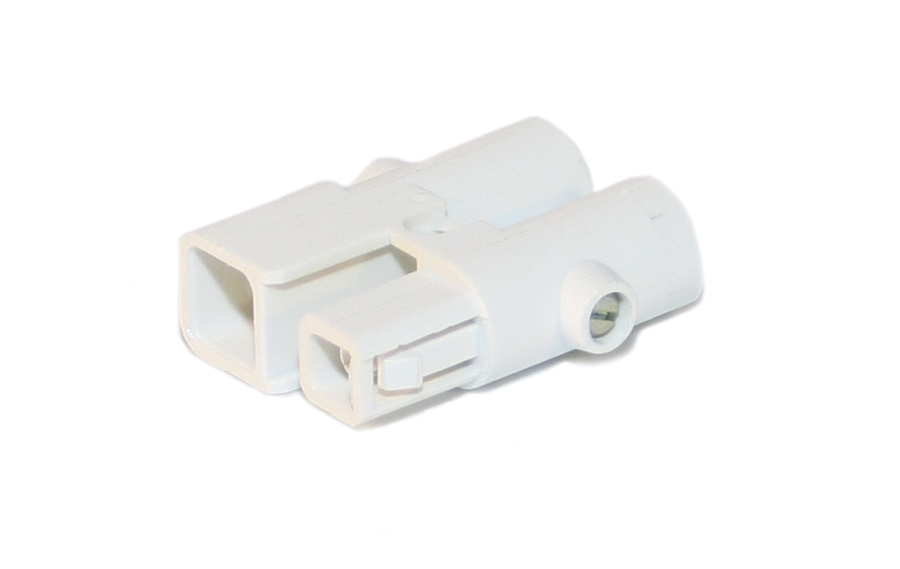
\includegraphics[scale=0.2]{images/wielandstekker}}
\item een voedingsadaptor 12 volt (verschillende vermogens)
\item een dimmer
\end{itemize}

De hoekprofielen met verlichting kunnen doorgekoppeld worden, let hierbij op de kleuren van de kabels!
Let op de stroomverdeling: de verlichting verbruikt ongeveer 1,25 Amp\`ere per meter. Dit houdt in dat het aantal te koppelen verlichtingsprofielen afhankelijk is van de gebruikte voedingsadaptor:
\\

\begin{tabular}{| l | l | l |}
\hline
Vermogen voeding&Amp\`erage&Aantal modules\\
\hline
36W&3A&2\\
\hline
60W&5A&4\\
\hline
72W&6A&4\\
\hline
120W&10A&8\\
\hline
\end{tabular}
\\

Bij overschrijding van de maximale stroom gaan de meeste adaptors de spanning verminderen, waardoor dus de totale verlichting zwakker gaat branden.
De LEDstrips worden als volgt gemonteerd:
\begin{itemize}
\item Deel de LEDstrip op in secties van 100cm.
\item Sluit aan elke kant een stuk wit aansluitsnoer (2 x 1mm$^{2}$) van ongeveer 50cm aan op de sectie LEDstrip, let hierbij op de kleuren: rood is +, blauw is -.
\item Isoleer de verbinding met het snoer met een stuk krimpkous (wit, 10mm diameter).
\item Plak de LEDstrip aan de binnenkant van het hoekprofiel, zo dicht mogelijk tegen de hoek aan.
\item Maak de beide uiteinden van de LEDstrip mechanisch vast aan het hoekprofiel met bijvoorbeeld tie-wraps of binddraad.
\item Monteer de Wieland stekkers aan de aansluitsnoeren.
\end{itemize}

\chapter{Het leggen van de rails}
\label{ch:rails}

Het leggen van de rails dient zo nauwkeurig mogelijk te gebeuren, anders is de kans op ontsporing of kortsluiting groot! Hierbij wordt gebruik gemaakt van de hartlijn die op de bovenkant van het baan\trace is aangebracht.
Het hart van de rails ligt op 28,5 mm van de hartlijn. Nu wordt eerst deze hartlijn op het baan\trace getekend.

\section{Gebruikte rail}
Voor een standaard module van 1200 mm gebruiken we een standaard \marklin \ flexibele K-rail van 900mm (\marklin \ artikelnummer 2205), plus 2 x een vaste lengte van 180mm (\marklin \ artikelnummer 2200).

\section{Montage}
Zoals genoemd wordt de flexrail in het midden gemonteerd, en de 2 vaste lengtes worden aan beide zijden van de flexrail vastgezet met standaard railverbinders en de standaard klemmetjes voor het verbinden van de middenrail. Hierna worden deze laatste klemmetje aan elkaar gesoldeerd:

\begin{itemize}
\item leg de complete constructie plat op een tafel, met de rails aan de onderkant, zodat de metalen strip voor de middenrail boven ligt.
\item Soldeer de lipjes van de midenrail aan beide zijden aan elkaar, zodat er zowel mechanisch als elektrisch een solide verbinding ontstaat.
\item Soldeer minimaal 2 draden aan de middenrail, elk aan een kant van de bak. Gebruik hiervoor een rode draad. Hiervoor moet het metaal worden blootgelegd middels een slijpschijfje (dremel), en als hulpmiddel voor het solderen kan verdund fosforzuur (Godfather Models \& Supply) gebruikt worden.
\end{itemize}

Wanneer deze draden zijn vast gesoldeerd wordt de rails op het baan\trace gelegd en met markeerspelden vastgezet. Deze spelden houden de rails op zijn plaats totdat deze zijn vastgelijmd. Bij de aansluitdraden wordt een klein gaatje geboord en de aansluitdraad door dit gaatje geschoven en strak getrokken. Wanneer de rails nu op de goede plaats ligt worden deze vastgelijmd. Voor het op de goede plaats leggen van de tweede rails maken we gebruik van een schuifmaat. Zie figuur \ref{figuur5}.

\begin{figure}[!ht]
  \captionbox
  {Afstellen rails\label{figuur5}}
  {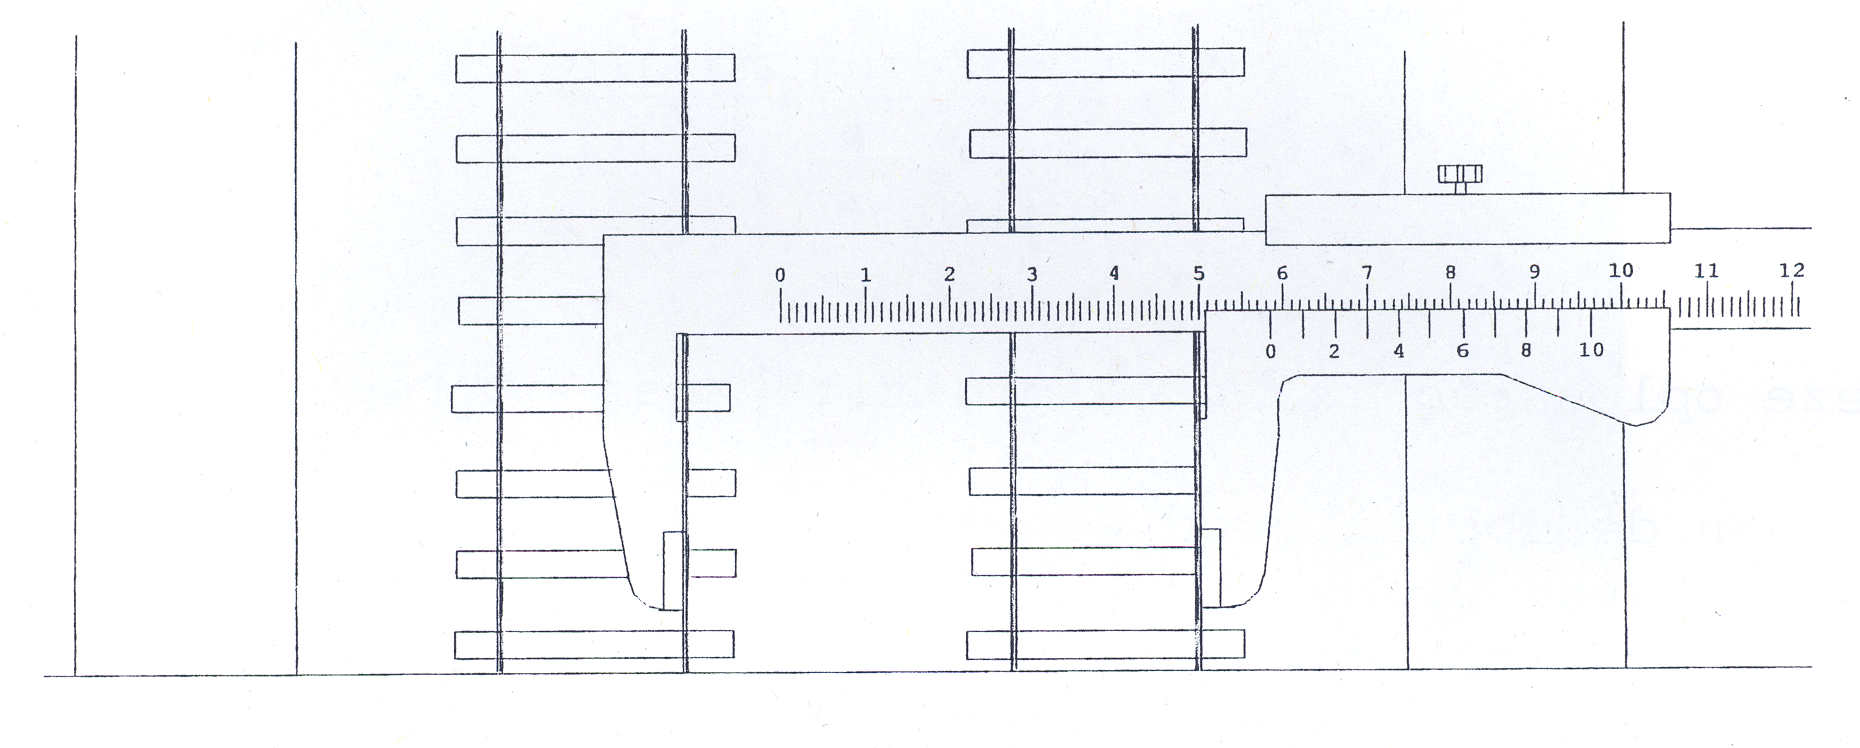
\includegraphics[scale=1.0]{images/rcu_figuur5}}
\end{figure}

De schuifmaat wordt ingesteld op 57 + 1.3 = 58,3 mm. De 57 mm is de hartafstand van de sporen en de 1,3 mm is de dikte van de spoorstaaf.
Ook de tweede rails wordt voor het leggen eerst voorzien van aansluitdraden alvorens deze wordt vastgelijmd.
Voor een extra stevige bevestiging aan het uiteinde wordt er in de laatste dwarsligger aan weerszijde een klein gaatje geboord. Hierdoor drukken we een klein spijkertje dat goed vast komt te zitten in het multiplex van het kopschot. Hiervoor kan ook een markeerspeld gebruikt worden, dan is voorboren niet nodig.De rails wordt nu van ballast voorzien, dit zorgt ook voor de fixering van de rails op de module. Het is zaak om dit minimaal 1 dag te laten drogen.
Hierna kunnen de spoorstaven netjes afgezaagd worden en zodanig afgevijld dat zij precies gelijk met het kopschot eindigen. Als alles goed is gegaan zal het koppelen van twee modules geen problemen geven. Maar om geringe afwijkingen toch nog te kunnen opvangen worden de spoorstaven over een lengte van $\pm$ 15 mm aan de binnenzijde afgeschuind. Zie figuur \ref{figuur6}.

\begin{figure}[!ht]
  \captionbox
  {Afschuinen spoorstaven\label{figuur6}}
  {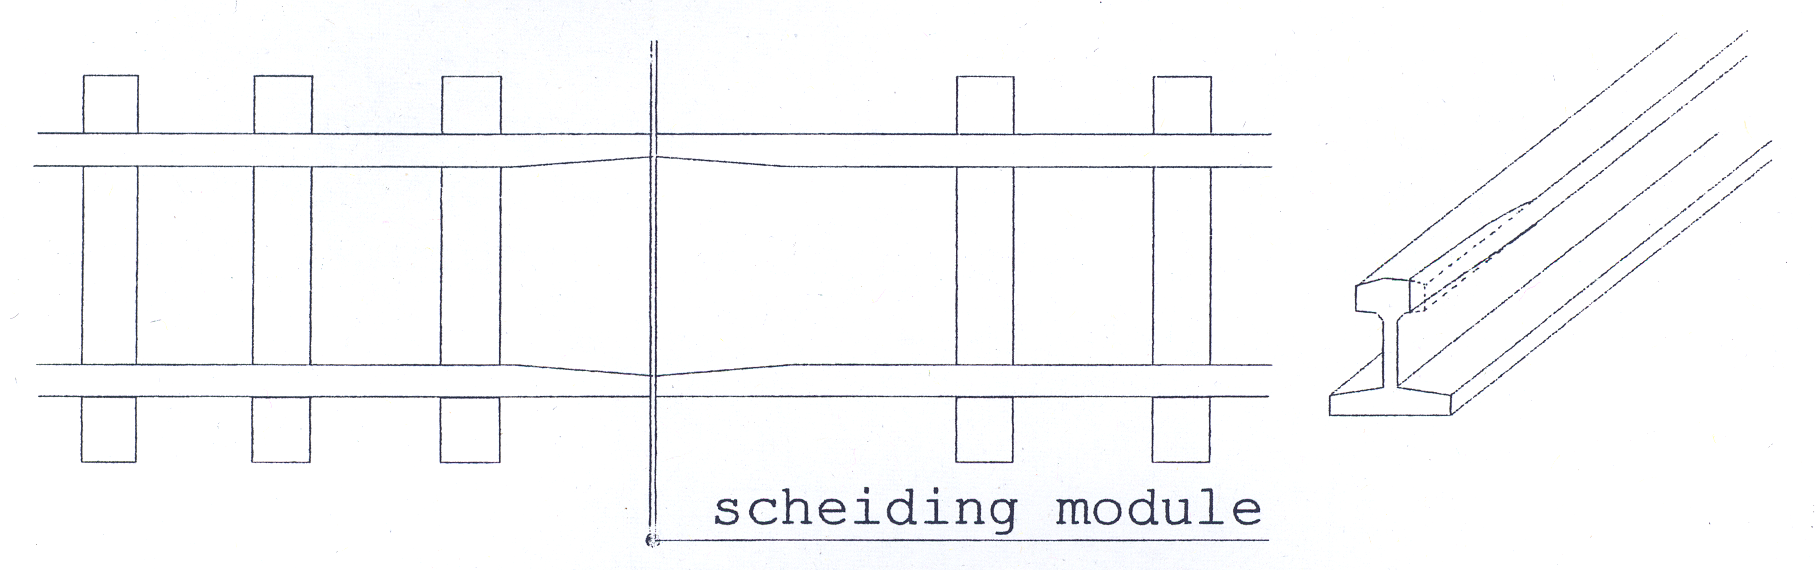
\includegraphics[scale=1.0]{images/rcu_figuur6}}
\end{figure}

Deze oplossing is in de praktijk zeer betrouwbaar gebleken.

Liggen de spoorstaven goed dan kunnen de draden aan de spoorstaven worden gesoldeerd. Het solderen aan de spoorstaven vraagt enige voorbereiding. Eerst moet op de plaats waar later gesoldeerd wordt de spoorstaaf schoon geschuurd worden. Daarna wordt met gebruikmaking van verdund fosforzuur een klein beetje soldeertin op de spoorstaaf aangebracht. Hierna wordt het vooraf vertinde draadje aan de spoorstaaf vast gesoldeerd. Vervolgens wordt een klein gaatje naast de rails geboord en het draadje er doorheen geschoven. Nu steken er onder uit het hout van het baan\trace drie draden, een rode, een bruine en een zwarte.

\section{Proef met Peco rail}

Bij wijze van proef wordt er gekeken of Pecorails met midden contactrail stevig genoeg zijn om de Marklin Rails te vervangen op de bakken. We maken gebruik van de volgende items:

\begin{itemize}
\item H0 - Code 100 - Rechte rail - L=670 mm (4x standaard lengte) artikelnummer: PEP-ST204 (figuur \ref{pecost204})
\item H0 - Code 100 - Flexrail met betonnen bielzen - L=914mm - nieuw zilver artikelnummer: PEP-SL0102 (figuur \ref{pecosl102})
\item H0 - Contactstrip voor 3-rail (wisselstroom) - voor wissels en kruisingen - L=1219 mm (voor code 75 en 100) artikelnummer: PEP-SL0018 (figuur \ref{pecosl18})
\end{itemize}

We gebruiken dan dus 2 x de ST-204 lengtes voor de rails met houten bielzen, of de flexrail SL-102 voor de rails met betonnen bielzen (hier zijn geen vaste lengtes voor beschikbaar).

\begin{figure}
\centering
\begin{subfigure}{.5\textwidth}
  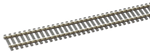
\includegraphics[scale=1.0]{images/rcu_peco_st204}
  \caption{Peco ST-204\label{pecost204}}
\end{subfigure}%
\begin{subfigure}{.5\textwidth}
  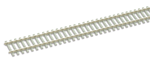
\includegraphics[scale=1.0]{images/rcu_peco_sl102}
  \caption{Peco SL-102\label{pecosl102}}
\end{subfigure}
\caption{Peco rails}
\end{figure}

\begin{figure}[!ht]
  \captionbox
  {Peco SL-18\label{pecosl18}}
  {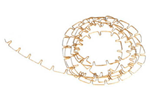
\includegraphics[scale=1.0]{images/rcu_peco_sl18}}
\end{figure}

\section{Proef met railplaatjes}

Om de aansluiting tussen de bakken te verbeteren gaan we een proef doen met zogenaamde 'railplaatjes', kleine printplaatjes waarop de einden van de rails worden gesoldeerd. Hierbij is de afstand tussen de rails geborgd op 57 mm, en is er dus ook een goede mechanische bevestiging van de rails geregeld.

\begin{figure}[!ht]
  \captionbox
  {Railplaatjes\label{railplaatjes}}
  {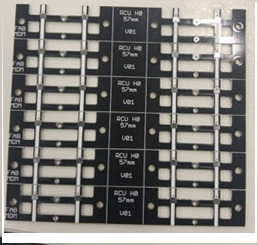
\includegraphics[scale=0.6]{images/railplaatjes}}
\end{figure}

\begin{figure}[!ht]
  \captionbox
  {Railplaatjes Gemonteerd op 2 vaste K-rails\label{railplaatjes_gemonteerd}}
  {\includegraphics[scale=0.2]{images/railplaatjes_gemonteerd}}
\end{figure}

Let op: bij monteren van de railplaatjes wordt de rechte kant aan het kopschot gemonteerd, de rails moeten daar worden afgezaagd zodat de overgang mechanisch zo sterk mogelijk is. Op afbeelding \ref{railplaatjes_gemonteerd} is dit nog niet gebeurd.

\chapter{Normen elektrische installatie}
\label{ch:elektra}

De elektrische installatie bestaat uit twee delen.

\begin{itemize}
\item De 230 volt voeding van de baan.
\item het laagspanningsgedeelte van de baan.
\end{itemize}

\section{De 230 volt voeding van de baan}
Onder de baan mogen vanwege de veiligheid geen 230V-aansluitingen gemonteerd worden, dus alle elektronische apparatuur wordt gevoed met stekkertrafos, die aangesloten worden op stekkerblokken die onder de baan op de grond liggen.

\section{Het laagspanningsgedeelte van de baan}

Er lopen 4 draden tussen elke bak:
\begin{itemize}
\item Een rode draad: deze is voor het voeden van de treinen (Middenrails);
\item Een bruine draad: dit is de massa draad van de baan (buitenste railsstaaf), deze rails mag nergens onderbroken zijn.
\\
Deze twee draden worden verbonden middels Wieland ST16 stekkers.

\item Een grijze of violette draad, deze is voor de binnenste railstaaf van de achterste rails
\item Een gele draad, deze is voor de binnenste railstaaf van de voorste rails.\\
De laatste 2 draden worden aan groene banaanstekker-chassisdelen.verbonden.
\end{itemize}
Alles 1mm$^{2}$ (snoer). 

\subsection{Modules zonder wissels}
Er zijn 2 soorten basismodules zonder wissels: met en zonder seinen. De basismodule met seinen heeft 4 bezetmeldersecties.
De secties worden aangesloten aan een 4 mm chassisdeel, waar een banaanstekker in past.
Een basismodule zonder seinen heeft aan elke kant 2 van zulke aansluitingen, die links en rechts zijn doorverbonden, dus 2 secties.
Een basismodule met seinen heeft ook aan elke kant 2 aansluitingen, maar deze zijn niet doorverbonden, dus er zijn 4 secties.

\subsection{Modules met wissels}
Een module met wissels is ook een soort basismodule: ook hier zijn 4 bezetmeldersecties, waarbij het doorgaande spoor een sectie is, en het afbuigende spoor een andere. Voor het aansluiten is deze hetzelfde als een basismodule met seinen.
Een module met wissels heeft dus geen seinen, de seinen staan op de module voor de wissels, zodat een trein altijd stopt op deze module, en nooit op de module met wissels. De wissels kunnen dus kort na het begin van de module geplaatst worden.
Treinen op het afbuigende spoor rijden door op de module n\'{a} de module met wissels, en stoppen dus nooit op deze module.
De bediening van de wissels moet gebeuren door schakelaars op de module zelf, met behulp van een externe voeding. Deze mag niet uit de baanspanning worden gevoed. Deze schakelaars moeten 'puls'-schakelaars zijn, dus mogen niet in een vaste positie blijven staan.
Verder moet de bediening aan te sluiten zijn op een wisseldecoder, zodat de wissels ook digitaal bestuurd kunnen worden. Beide mogelijkheden moeten parallel inzetbaar zijn, dus zelfs met digitale besturing moet handbediening nog mogelijk zijn.
Er is alleen een tekening gemaakt van 1 variant, type '3a', zie figuur \ref{im:modulebak_seinen_wissels}. Desgewenst kunnen ook de andere varianten uitgetekend worden:

\begin{table}[!ht]
{\renewcommand{\arraystretch}{3}%
\begin{tabular}{| l | m{7cm} | m{7cm} |}
\hline
Basismodule 3a&Links 2 sporen, rechts 4 sporen& \parbox[c]{1em}{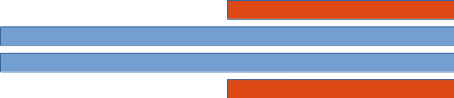
\includegraphics[width=7cm]{images/module_3a}} \\
\hline
Basismodule 3b&Links 4 sporen, rechts 2 sporen& \parbox[c]{1em}{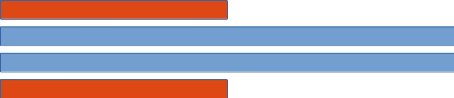
\includegraphics[width=7cm]{images/module_3b}} \\
\hline
Basismodule 3c&Links 2 sporen, rechts 3 sporen (linkerspoor met wissel)&\parbox[c]{1em} {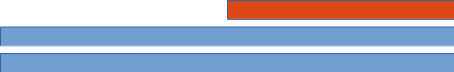
\includegraphics[width=7cm]{images/module_3c}} \\
\hline
Basismodule 3d&Links 2 sporen, rechts 3 sporen (rechterspoor met wissel)&\parbox[c]{1em} {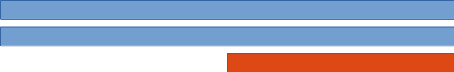
\includegraphics[width=7cm]{images/module_3d}} \\
\hline
Basismodule 3e&Links 3 sporen, rechts 2 sporen (linkerspoor met wissel)&\parbox[c]{1em} {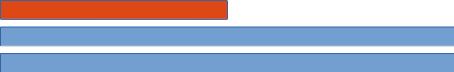
\includegraphics[width=7cm]{images/module_3e}} \\
\hline
Basismodule 3f&Links 3 sporen, rechts 2 sporen (rechterspoor met wissel)&\parbox[c]{1em} {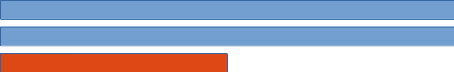
\includegraphics[width=7cm]{images/module_3f}} \\
\hline
Basismodule 3g&Links 3 sporen, rechts 3 sporen (linkerspoor met wissel naar links, rechterspoor met wissel naar rechts)&\parbox[c]{1em} {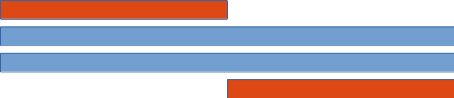
\includegraphics[width=7cm]{images/module_3g}} \\
\hline
Basismodule 3h&Links 3 sporen, rechts 3 sporen ( rechterspoor met wissel naar links, linkerspoor met wissel naar rechts)&\parbox[c]{1em} {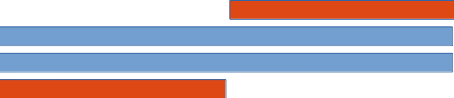
\includegraphics[width=7cm]{images/module_3h}} \\
\hline
\end{tabular}
}
\caption{Varianten Modulebak met wissels}
\end{table}

\subsection{Bezetmeldingsdraden, Remstukken en stopstukken}
Deze worden voorzien van  violet en grijs  0,5 mm$^{2}$ (kabel/massief tbv RJ45 chassis)

De doorsnede van de draden voor de ringleiding stopcontacten en stekker moet minimaal 0,65 mm$^{2}$ zijn, omdat anders een te groot spanningsverlies ontstaat of de draden worden te heet. Dikkere draad mag natuurlijk ook.
Het snoer tussen de bakken en de stekker moet van soepel draad zijn, en eveneens tenminste 0,65 mm$^{2}$ dik zijn.

De overgang van de ringleiding naar het snoer wordt gemaakt m.b.v. een kroonsteen. Omdat de sporen behalve via de stekkerverbinding op geen enkele andere wijze met elkaar verbonden zijn, moeten op elke module de sporen, op twee plaatsen per rails, met de ringleiding verbonden worden. De ringleiding moet separaat van de rails doorverbonden worden van het ene naar het andere eind van de bak. Zie figuur \ref{im:modulebak}.

Het is raadzaam om het snoer bij de kroonsteen van een trekontlasting te voorzien, om lostrekken van het snoer uit de kroonsteen te voorkomen.

Het op twee plaatsen aansluiten van de rails per module maakt de installatie bedrijfszekerder. Wanneer er ook in de transformator een beveiliging tegen kortsluiting is ingebouwd, voldoet de installatie aan de voorschriften die bij de vereniging gelden. Dit voorgaande geldt voor zowel gekochte als voor zelfbouw voedingen!

\section{Aansluiten Modules}
Op de volgende pagina's worden de aansluitingen per modulebak aangegeven.
Dit zijn de aansluitschema's zoals besproken in het overleg van woensdag 30 april 2016 met de aanwezige leden van de H0-groep, waaronder de moduleco\"{o}rdinatoren (Marc en Peter).
Er is besloten om af te stappen van de PTT-stekers en een versimpelde aansluiting te gebruiken met de Wieland ST16 stekkers die ook gebruikt worden voor de BNLS-modules, deze zijn geschikt voor 48V/25A, goedkoop (ca. 1 euro per stuk), en simpel aan te sluiten middels schroefaansluitingen (zie figuur \ref{im:wielandstekker})

\begin{figure}[!ht]
  \captionbox
  {Wieland ST16/2 stekker\label{im:wielandstekker}}
  {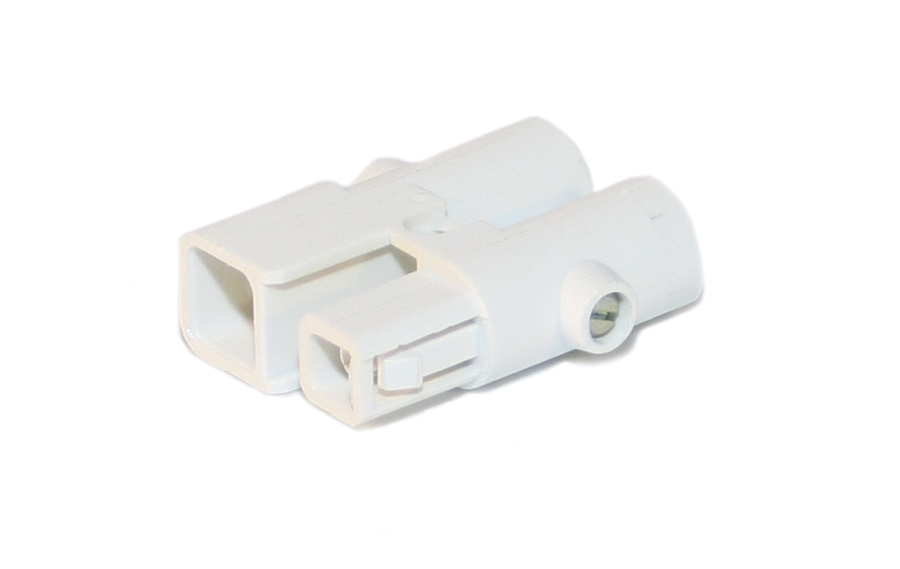
\includegraphics[scale=0.2]{images/wielandstekker}}
\end{figure}

\subsection{Kabels}
De kleuren van de kabels zijn niet kritisch, het is alleen voor het troubleshooten nuttig om de aangegeven kleuren aan te houden.

\begin{figure}[!ht]
  \captionbox
  {Bovenaanzicht bekabeling basismodule\label{im:modulebak}}
  {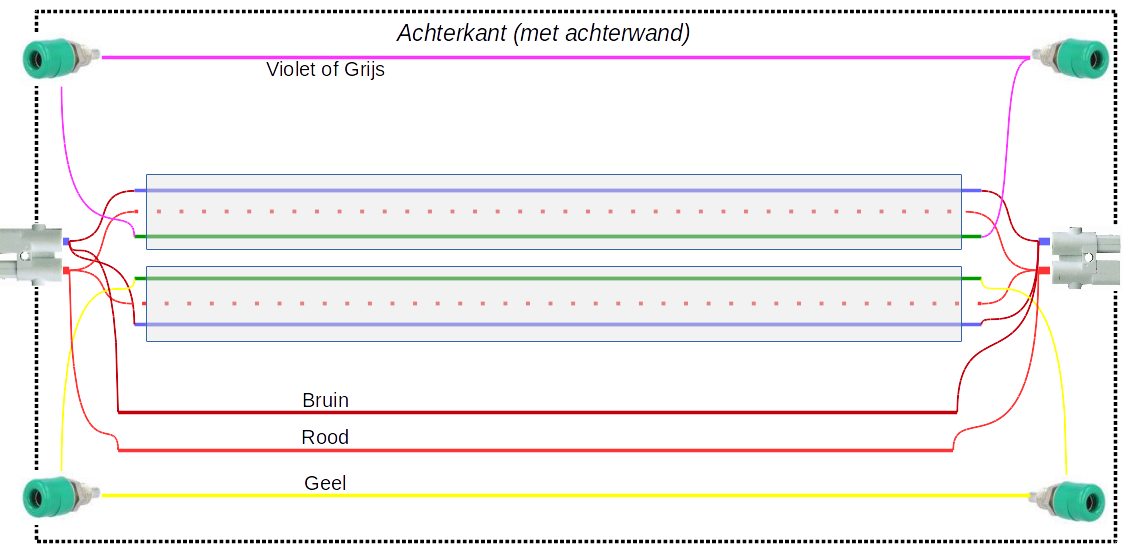
\includegraphics[scale=0.6]{images/rcu_modulebak}}
\end{figure}

\begin{figure}[!ht]
  \captionbox
  {Bovenaanzicht bekabeling seinenmodule\label{im:modulebak_seinen}}
  {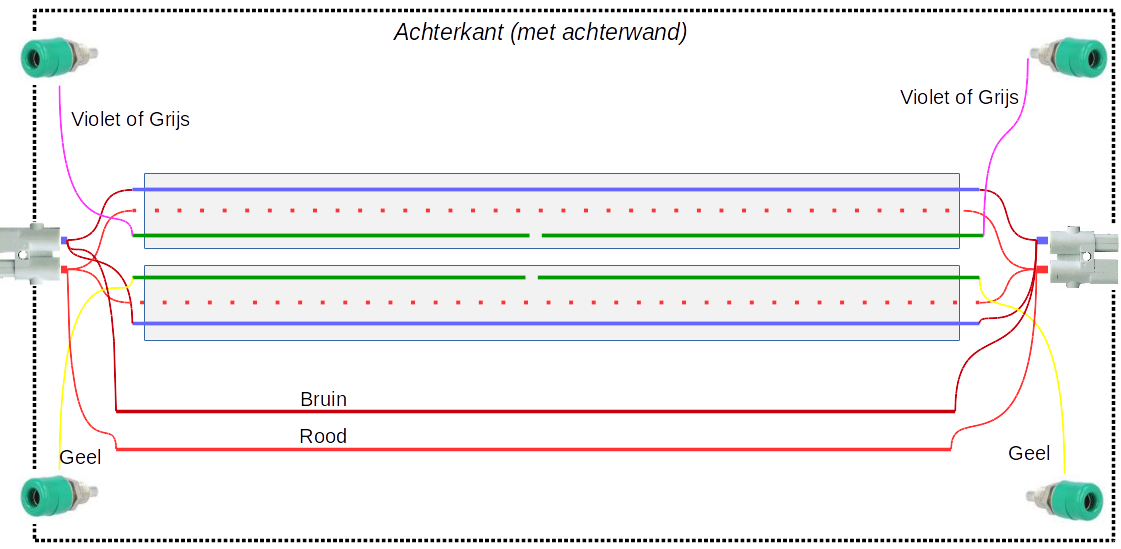
\includegraphics[scale=0.6]{images/rcu_modulebak_seinen}}
\end{figure}

\begin{figure}[!ht]
  \captionbox
  {Bovenaanzicht bekabeling seinenmodule met wissels\label{im:modulebak_seinen_wissels}}
  {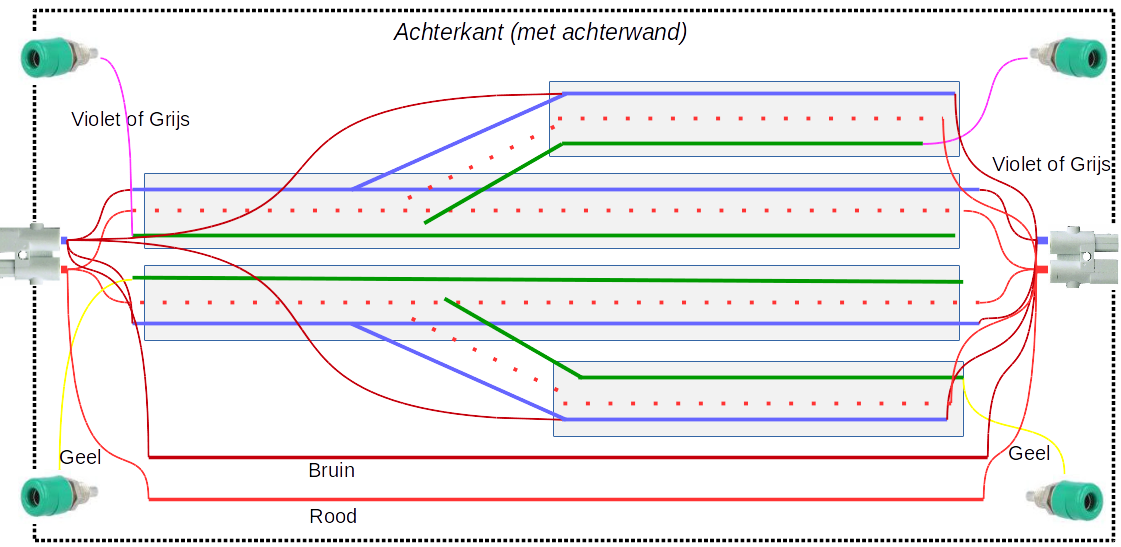
\includegraphics[scale=0.6]{images/rcu_modulebak_seinen_wissels}}
\end{figure}

\chapter{Wissels en Seinen}
\label{ch:beveiliging}

\section{Wisselaansturing}
Voor het bedienen van de wissels wordt geen gebruik gemaakt van relais die de fabrikant van de wissels levert, daar deze kwetsbaar zijn en veel storingen veroorzaken. Er is gekozen voor het gebruik van servo's. Hiervoor wordt gebruik gemaakt van standaard modelbouwservo's en een aantal stukjes styreen om een standaard servohouder te maken. De aansturing van de servo's gebeurt met een op Arduino gebaseerde print. Deze maakt het mogelijk om 2 servos's aan te sturen, waarbij per servo de begin- en eindpositie kan worden ingesteld, alsmede de snelheid waarmee de wissel omgezet wordt. Het bedienen van de wissels gebeurt met 2 drukknoppen per servo, waarbij parallel een wisseldecoder kan worden ingezet om de wissels digitaal aan te kunnen sturen.

\section{Seinen}

De treinenloop wordt op de baan geregeld m.b.v. seinen en de daarbij behorende rem- en stop stukken.

Wanneer een trein een sein passeert moet dit sein automatisch in de stand stop komen,
stand stop is een rood tonend sein.

Bij een station moet zowel het inrijden als het uitrijden beveiligd worden met een sein. Het op ''groen'' zetten van een sein kan op verschillende manieren worden gedaan. Volautomatisch, niet zo geschikt voor seinen die een gevarenpunt beveiligen, of handmatig.
Een gevarenpunt is bijvoorbeeld een inrij- of uitrijsein van een station of bij een spooraftakking. Er is echter een mogelijkheid om bij de hoofdsporen een tijdelijk automatisch groen in te bouwen zodat niet altijd alles handmatig bediend moet worden.
\section{Aansturing Seinen}

\begin{figure}
  \centering
  \begin{subfigure}{.5\textwidth}
    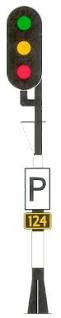
\includegraphics[scale=0.6]{images/henckes_p_sein}
    \caption{Henckes P-Sein\label{im:psein}}
  \end{subfigure}%
  \begin{subfigure}{.5\textwidth}
    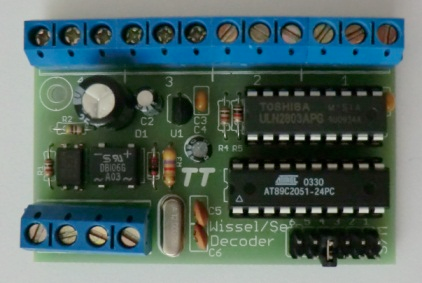
\includegraphics[scale=0.6]{images/seindecoder}
    \caption{Traintech Wissel/Seindecoder\label{im:seindecoder}}
  \end{subfigure}
  \caption{Gebruikte P-seinen en sturing}
\end{figure}

Hoewel er speciale decoders zijn voor het aansturen van allerlei lichtseinen, is het voor het gebruik van nederlandse lichtseinen zonder cijferbak (P-seinen) een simpeler oplossing mogelijk: schakeldecoders met 2 uitgangen. Hierbij wordt gebruik gemaakt van het feit dat de twee uitgangen van een schakeldecoder in principe 4 verschillende mogelijkheden kunnen uitbeelden, wat ruim voldoende is voor de 3 mogelijkheden van een P-sein. Hierbij worden de extra seinbeelden zoals 'geel knipper' e.d. niet gebruikt.
We gebruiken hiervoor de '4-voudige wissel/sein decoder' van traintech (webshop.traintech.nl), met een 'diodetruc':
Er wordt hierbij een extra aansluiting gemaakt aan de min-aansluiting van de print, dit is het printspoor wat aan de buitenkant loopt. Hier worden 2 in serie geschakelde diodes (1N4148) aan gesoldeerd, waarna deze aan de rode LED van het sein wordt aangesloten (zie figuur \ref{im:aansturing_sein}).

\begin{figure}[!ht]
  \centering
  \begin{subfigure}{.5\textwidth}
    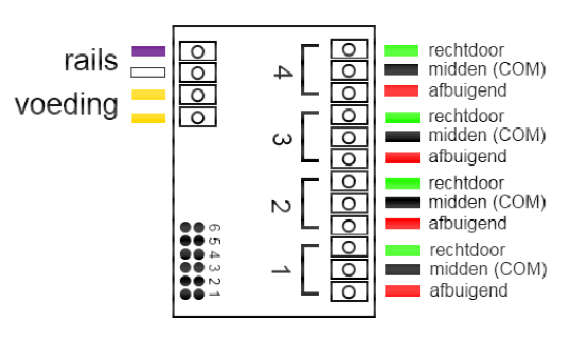
\includegraphics[scale=0.4]{images/traintech_decoder}
    \caption{Traintech Decoder\label{im:traintech_decoder}}
  \end{subfigure}%
  \begin{subfigure}{.5\textwidth}
    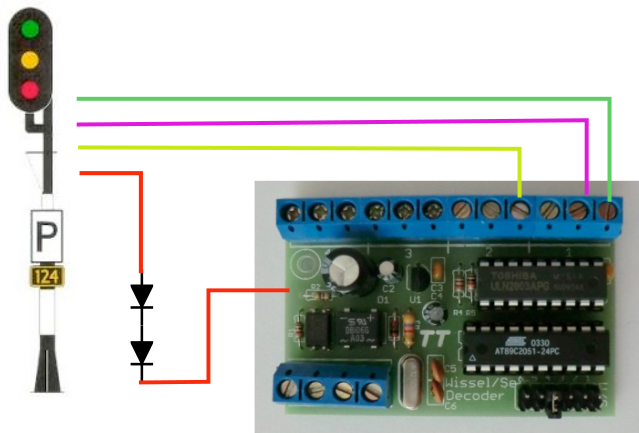
\includegraphics[scale=0.5]{images/aansluiting_seinen}
    \caption{Aansluiten decoder\label{im:aansturing_sein}}
   \end{subfigure}
   \caption{Seindecoders}
\end{figure}

Op 1 decoder kunnen op deze manier 2 seinen worden aangesloten.
De voeding van de decoder kan zowel door het digitale signaal als door een aparte voeding worden geleverd, zie hiervoor de handleiding van de decoder.
Er wordt hierbij een extra aansluiting gemaakt aan de min-aansluiting van de print, dit is het printspoor wat aan de buitenkant loopt. Hier worden 2 in serie geschakelde diodes (1N4148) aan gesoldeerd, waarna deze aan de rode LED van het sein wordt aangesloten.
Op 1 decoder kunnen op deze manier 2 seinen worden aangesloten.
De voeding van de decoder kan zowel door het digitale signaal als door een aparte voeding worden geleverd, zie hiervoor de handleiding van de decoder.

Dus bij het aansturen van het sein geldt:
\begin{enumerate}
\item uitgang 1 afbuigend, uitgang 2 recht: groen
\item uitgang 1 recht, uitgang 2 afbuigend: geel
\item uitgang 1 en 2 recht: rood
\item uitgang 1 en 2 afbuigend: nvt
\end{enumerate}

\chapter{De bovenleiding}
\label{ch:bovenleiding}

Voor de bovenleiding wordt het materiaal van Sommerfeldt of van Viessmann gebruikt. We houden uiteraard zoveel mogelijk het Nederlandse voorbeeld aan. Maar soms is de situatie zodanig dat er andere oplossingen bedacht moeten worden. Dan is een Duitse oplossing eventueel mogelijk. Uiteraard wordt getracht dit te zoveel mogelijk te voorkomen. De rijdraden worden niet elektrisch aangesloten. Ze dienen overigens wel zodanig opgehangen te worden, dat treinen met stroomafnemers omhoog 5mm onder de draad kunnen rijden. Om het aanzien van de baan ten goede te laten komen, wordt er voor de rijdraden gebruik gemaakt van de standaard rijdraad van Sommerfeldt/Viessmann. De plaats van de masten is conform de montagevoorschriften van Sommerfeldt. Dat wil zeggen, 34 mm uit het hart van het spoor en 69 mm boven het spoor. De afstand van de mast tot de scheiding van de module bedraagt precies 135 mm. Als overgangsrijdraad tussen twee modules dient een Sommerfeldt/Viessmann rijdraad. Deze heeft een lengte van 270 mm, waarvan de uiteinden gebogen zijn, als in figuur \ref{figuur9}. Deze normen zijn uiteraard belangrijk, maar ten alle tijden moet bekeken worden of de trein zonder problemen onder de bovenleiding kan passeren. Dat is veel belangrijker dan dat een bovenleiding er realistisch uitziet!

\begin{figure}[!ht]
  \captionbox
  {Sommerfeldt rijdraad\label{figuur9}}
  {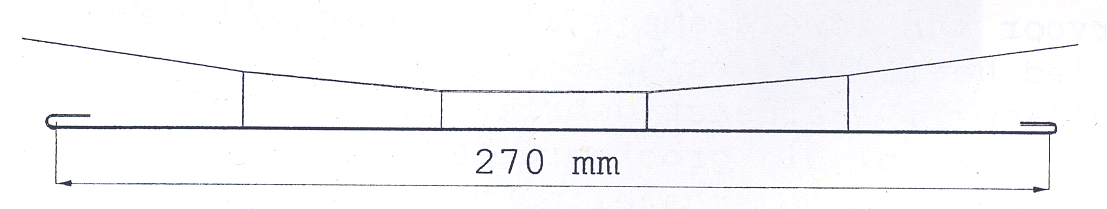
\includegraphics[scale=1.0]{images/rcu_figuur9}}
\end{figure}

De rijdraad wordt zigzaggend boven de rails opgehangen. Om de zigzag ophanging van de rijdraad ook bij de overgang van de module voort te zetten, dient in de rijrichting gezien de eerste mast een lange uitlegger te hebben en de laatste een korte. Voor NS-portaalmasten houdt dit in, dat voor het rechterspoor de uithouder aan de V-steun is gemonteerd en de uithouder van het linkerspoor aan de linkermast. Zie figuur \ref{figuur10}.

\begin{figure}[!ht]
  \captionbox
  {Zigzaggende rijdraad\label{figuur10}}
  {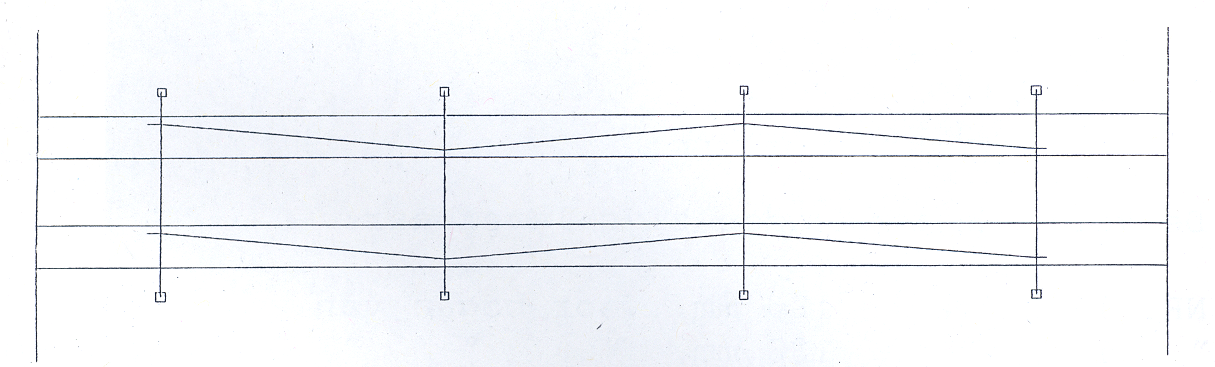
\includegraphics[scale=1.0]{images/rcu_figuur10}}
\end{figure}

Een uitzondering hierop vormen de hoekmodules. In een boog dient voor het buitenste spoor altijd een korte uithouder en voor het binnenste spoor een lange uithouder toegepast te worden. Dit houdt in dat aan de ene zijde de opstelling wel klopt maar aan de andere zijde niet.

Zie paragraaf \ref{ch:normen_bovenleiding} voor benodigde onderdelen en nummers

\section{Normen bovenleiding}
\label{ch:normen_bovenleiding}

\begin{table}[!ht]
\begin{tabular}{| l | l |}
\hline
\cellcolor[gray]{0.84}Hoogte rijdraad&69 mm t.o.v. bovenkant spoorstaaf\\
\hline
\cellcolor[gray]{0.84}Plaats mast&34 mm uit het hart van de rail\\
\hline
\cellcolor[gray]{0.84}Plaats eerste en laatste mast&135 mm van de rand van de bak\\
\hline
\cellcolor[gray]{0.84}Overgangsrijdraad&Sommerfeldt nr. 145 (270 mm)\\
\hline
\cellcolor[gray]{0.84}Uitslag rijdraad&6 mm naar weerszijde\\
\hline
\end{tabular}
\caption{Normen bovenleiding}
\end{table}

Bij een rechte bak, in de rijrichting gezien, is aan het eerste portaal de rijdraad bevestigd aan de Y-hanger en aan het tweede portaal aan de mast zelf.
Bij een hoekbak is de rijdraad in de buitenboog bevestigd aan de mast en bij de binnenboog aan de Y-hanger.

Uit het programma van Sommerfeldt worden de volgende masten en portalen gebruikt:

\begin{table}[!ht]
\begin{tabular}{| l |p{8cm}|}
\hline
\cellcolor[gray]{0.84}Nr. 500&Losse mast\\
\hline
\cellcolor[gray]{0.84}Nr. 520&Mast met \'{e}\'{e}n uitlegger voor enkelspoor\\
\hline
\cellcolor[gray]{0.84}Nr. 570&Portaal voor twee sporen\\
\hline
\cellcolor[gray]{0.84}Nr. 580&Portaal voor drie sporen\\
\hline
\cellcolor[gray]{0.84}Nr. 509&Spaninrichting\\
\hline
\cellcolor[gray]{0.84}Nr. 504&Isolatorbruggen\\
\hline
\cellcolor[gray]{0.84}Nr. 505&Isolatoren\\
\hline
\cellcolor[gray]{0.84}Nr. 163&Mastschakelaar\\
\hline
\end{tabular}
\caption{Sommerfeldt artikelnummers}
\end{table}

De volgende rijdraden zijn leverbaar:

\begin{table}[!ht]
\begin{tabular}{| l | l | l |}
\hline
\cellcolor[gray]{0.84}Nr. 140&Lengte 180 mm&Voor bogen vanaf R 300 mm\\
\hline
\cellcolor[gray]{0.84}Nr. 141&Lengte 188 mm&Voor bogen vanaf R 340 mm\\
\hline
\cellcolor[gray]{0.84}Nr. 142&Lengte 215 mm&Voor bogen vanaf R 420 mm\\
\hline
\cellcolor[gray]{0.84}Nr. 143&Lengte 229 mm&Voor bogen vanaf R 500 mm\\
\hline
\cellcolor[gray]{0.84}Nr. 144&Lengte 250 mm&Voor bogen vanaf R 600 mm\\
\hline
\cellcolor[gray]{0.84}Nr. 145&Lengte 270 mm&Voor bogen vanaf R 700 mm\\
\hline
\cellcolor[gray]{0.84}Nr. 146&Lengte 315 mm&Voor bogen vanaf R 900 mm\\
\hline
\cellcolor[gray]{0.84}Nr. 147&Lengte 360 mm&Voor bogen vanaf R 1200 mm\\
\hline
\cellcolor[gray]{0.84}Nr. 148&Lengte 375 mm&\\
\hline
\cellcolor[gray]{0.84}Nr. 149&Lengte 450 mm&\\
\hline
\cellcolor[gray]{0.84}Nr. 160&Lengte 500 mm&\\
\hline
\end{tabular}
\caption{Sommerfeldt Rijdraden}
\end{table}

\chapter{Opbouw van het landschap}
\label{ch:landschap}

Het landschap dient een Nederlandse uitstraling te hebben met Nederlandse gebouwen en toebehoren.

De ondergrond van het landschap bestaat uit een raamwerk van hout dat in de vorm van het landschap is gezaagd. Over dit raamwerk wordt horrengaas gelegd en vastgezet met nietjes. Over dit gaas wordt een laag alabastine aangebracht. Vooraf wordt de alabastine gemengd met kleurpigment. Bijvoorbeeld de kleur van klei, zand of veen. Hierdoor ontstaan er geen witte plekken in het landschap. B.v. als er geboord moet worden. Ook is het dan niet nodig het hele landschap te schilderen.
Een voorbeeld van een houten raamwerk is te zien in figuur \ref{figuur11}.

\begin{figure}[!ht]
  \captionbox
  {Houten raamwerk\label{figuur11}}
  {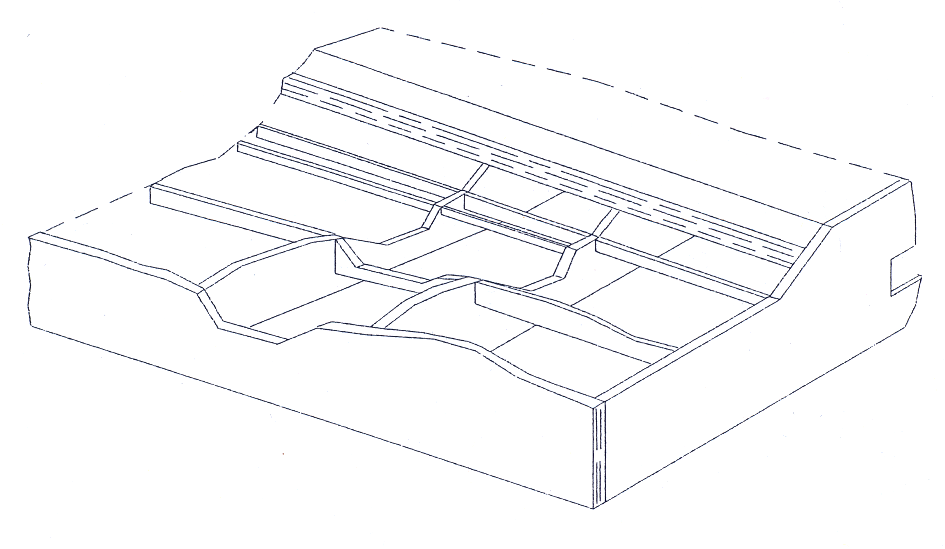
\includegraphics[scale=1.0]{images/rcu_figuur11}}
\end{figure}

Op plaatsen waar een grote boom of gebouw komt te staan wordt horizontaal een plankje in het raamwerk aangebracht, dit om een goede bevestiging mogelijk te maken.
Bij de onderkant van een sloot of rivier breng ik ook een plaatje multiplex aan om bruggetjes of kademuren op te bevestigen. Tijdens de opbouw is het erg belangrijk om de modulebak goed waterpas neer te zetten en zodat alles goed in het lood en waterpas komt te staan. Niets is zo storend als b.v. een kademuur of een huis storend scheef staan. Ook bij het gieten van het water moet hierop gelet worden.

\section{Volgorde bij de opbouw van het landschap}

Het landschap wordt van onder naar boven opgebouwd.
Dit betekent dat eerst de sloten, daarna de wegen en de ondergrond van gebouwen en kunstwerken, bruggen en tunnels worden gemaakt.
Nu volgt de kruidenlaag, gras en lage planten, daarna de struiken en als laatste de bomen.
Waarbij eerst de kleine bomen en pas daarna de grote.
In figuur \ref{figuur12} is dit alles in een eenvoudig schema weergegeven.

\begin{figure}[!ht]
  \captionbox
  {Opbouw landschap\label{figuur12}}
  {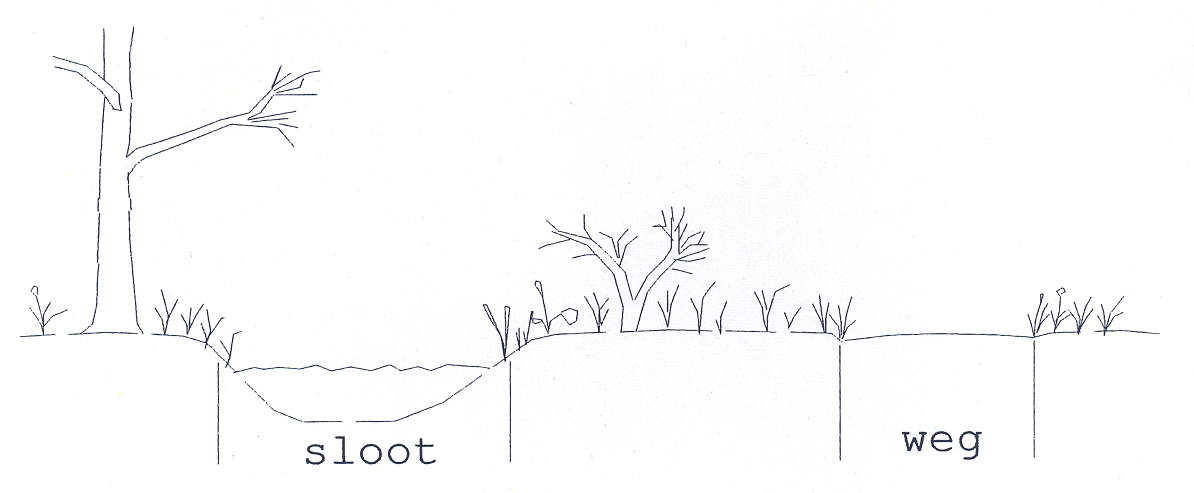
\includegraphics[scale=1.0]{images/rcu_figuur12}}
\end{figure}

Om de totale baan als een geheel te doen overkomen zijn er normen v.w.b. het materiaal en de kleuren die gebruikt worden om het landschap vorm te geven.

Het gebruik van gekleurd zaagsel is niet toegestaan. Ook zaken die niet op schaal zijn, b.v. auto's, figuren en huizen gebruiken we niet. Of b.v. ''borstels'' als bomen.

\section{Landschapsnormen}

Deze norm bevat de namen en nummers van de gebruikte fabrikanten binnen de M\"{a}rklinbaan bij Railclub Utrecht.

\begin{table}[!ht]
\begin{tabular}{| l | l |}
\hline
\cellcolor[gray]{0.84}Wegen van asfalt&Humbrol nr. 53\\
\hline
\cellcolor[gray]{0.84}Bovenleidingsportalen&Humbrol nr. 78\\
\hline
\cellcolor[gray]{0.84}'Roest' spoorstaven  worden twee kleuren&Humbrol nr. 113\\
\hline
\cellcolor[gray]{0.84}Telefoonkasten langs de vrije baan&Humbrol nr. 78\\
\hline
\cellcolor[gray]{0.84}Apparatenkasten langs de vrije baan&Humbrol nr. 78\\
\hline
\cellcolor[gray]{0.84}Ballastbed&Heki nr. 3155 of 3156\\
\hline
\cellcolor[gray]{0.84}Gras&Busch nr. 7111 of 7116\\
\hline
\cellcolor[gray]{0.84}Kruidenlaag&Heki, Busch of Woodland\\
\hline
\cellcolor[gray]{0.84}Struikenlaag&Heki, Busch of Woodland\\
\hline
\cellcolor[gray]{0.84}Het loof van de bomen&Heki, Busch of Woodland\\
\hline
\cellcolor[gray]{0.84}Ruig gras&heki\\
\hline
\end{tabular}
\caption{Onderdelen landschap}
\end{table}

Het spoor kan gelegen zijn op een spoordijk of loopt door een heuvel heen, dit noemen we een insnijding. Ook wanneer het spoor op maaiveld hoogte ligt, maaiveld is bovenzijde grond, zal het altijd iets hoger liggen dan de directe omgeving. Hierna volgen een voorbeeld van een spoordijk en een insnijding (figuur \ref{figuur13}).

\begin{figure}[!ht]
  \captionbox
  {Insnijdingen\label{figuur13}}
  {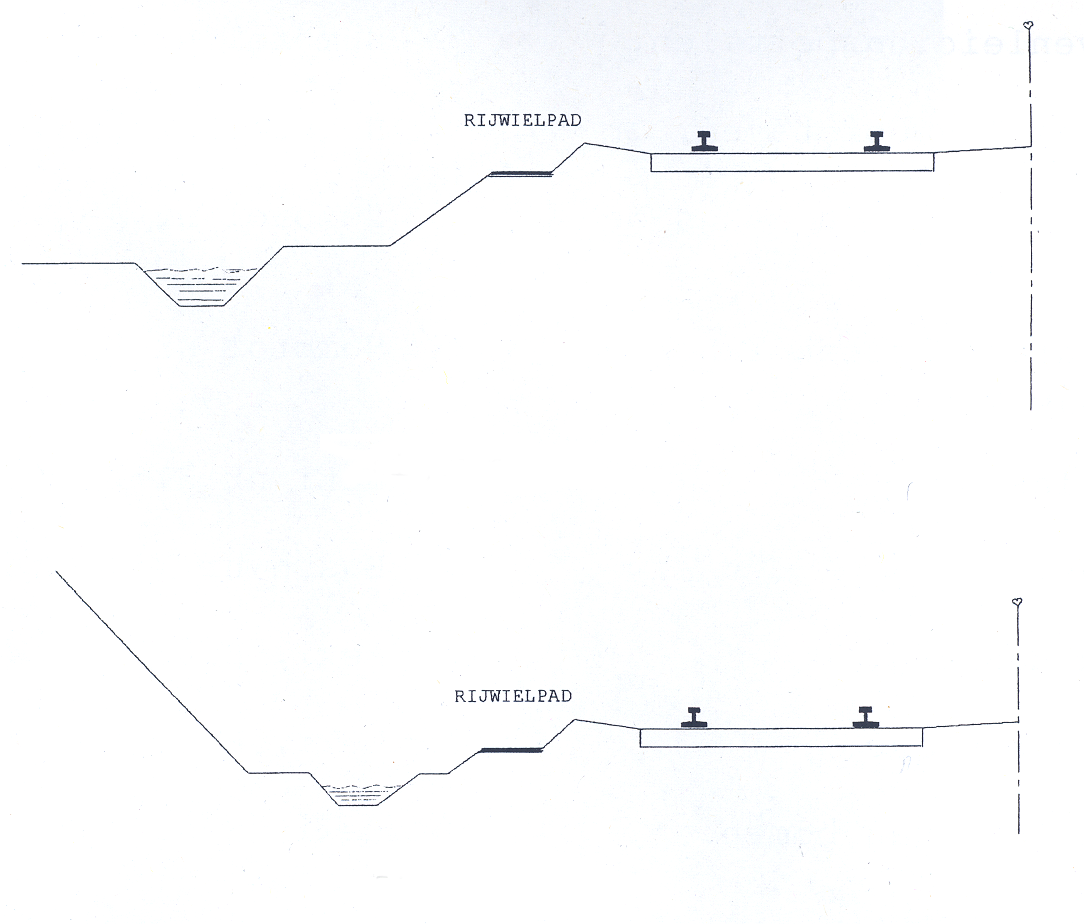
\includegraphics[scale=1.0]{images/rcu_figuur13_14}}
\end{figure}

In de figuren \ref{figuur15} en \ref{figuur16} zijn de maten aangegeven die in het stationsgebied zorgdragen voor het probleemloos passeren van de treinen langs perrons,seinen, gebouwen en bruggen.

\begin{figure}[!ht]
  \captionbox
  {Profiel vrije ruimte 1\label{figuur15}}
  {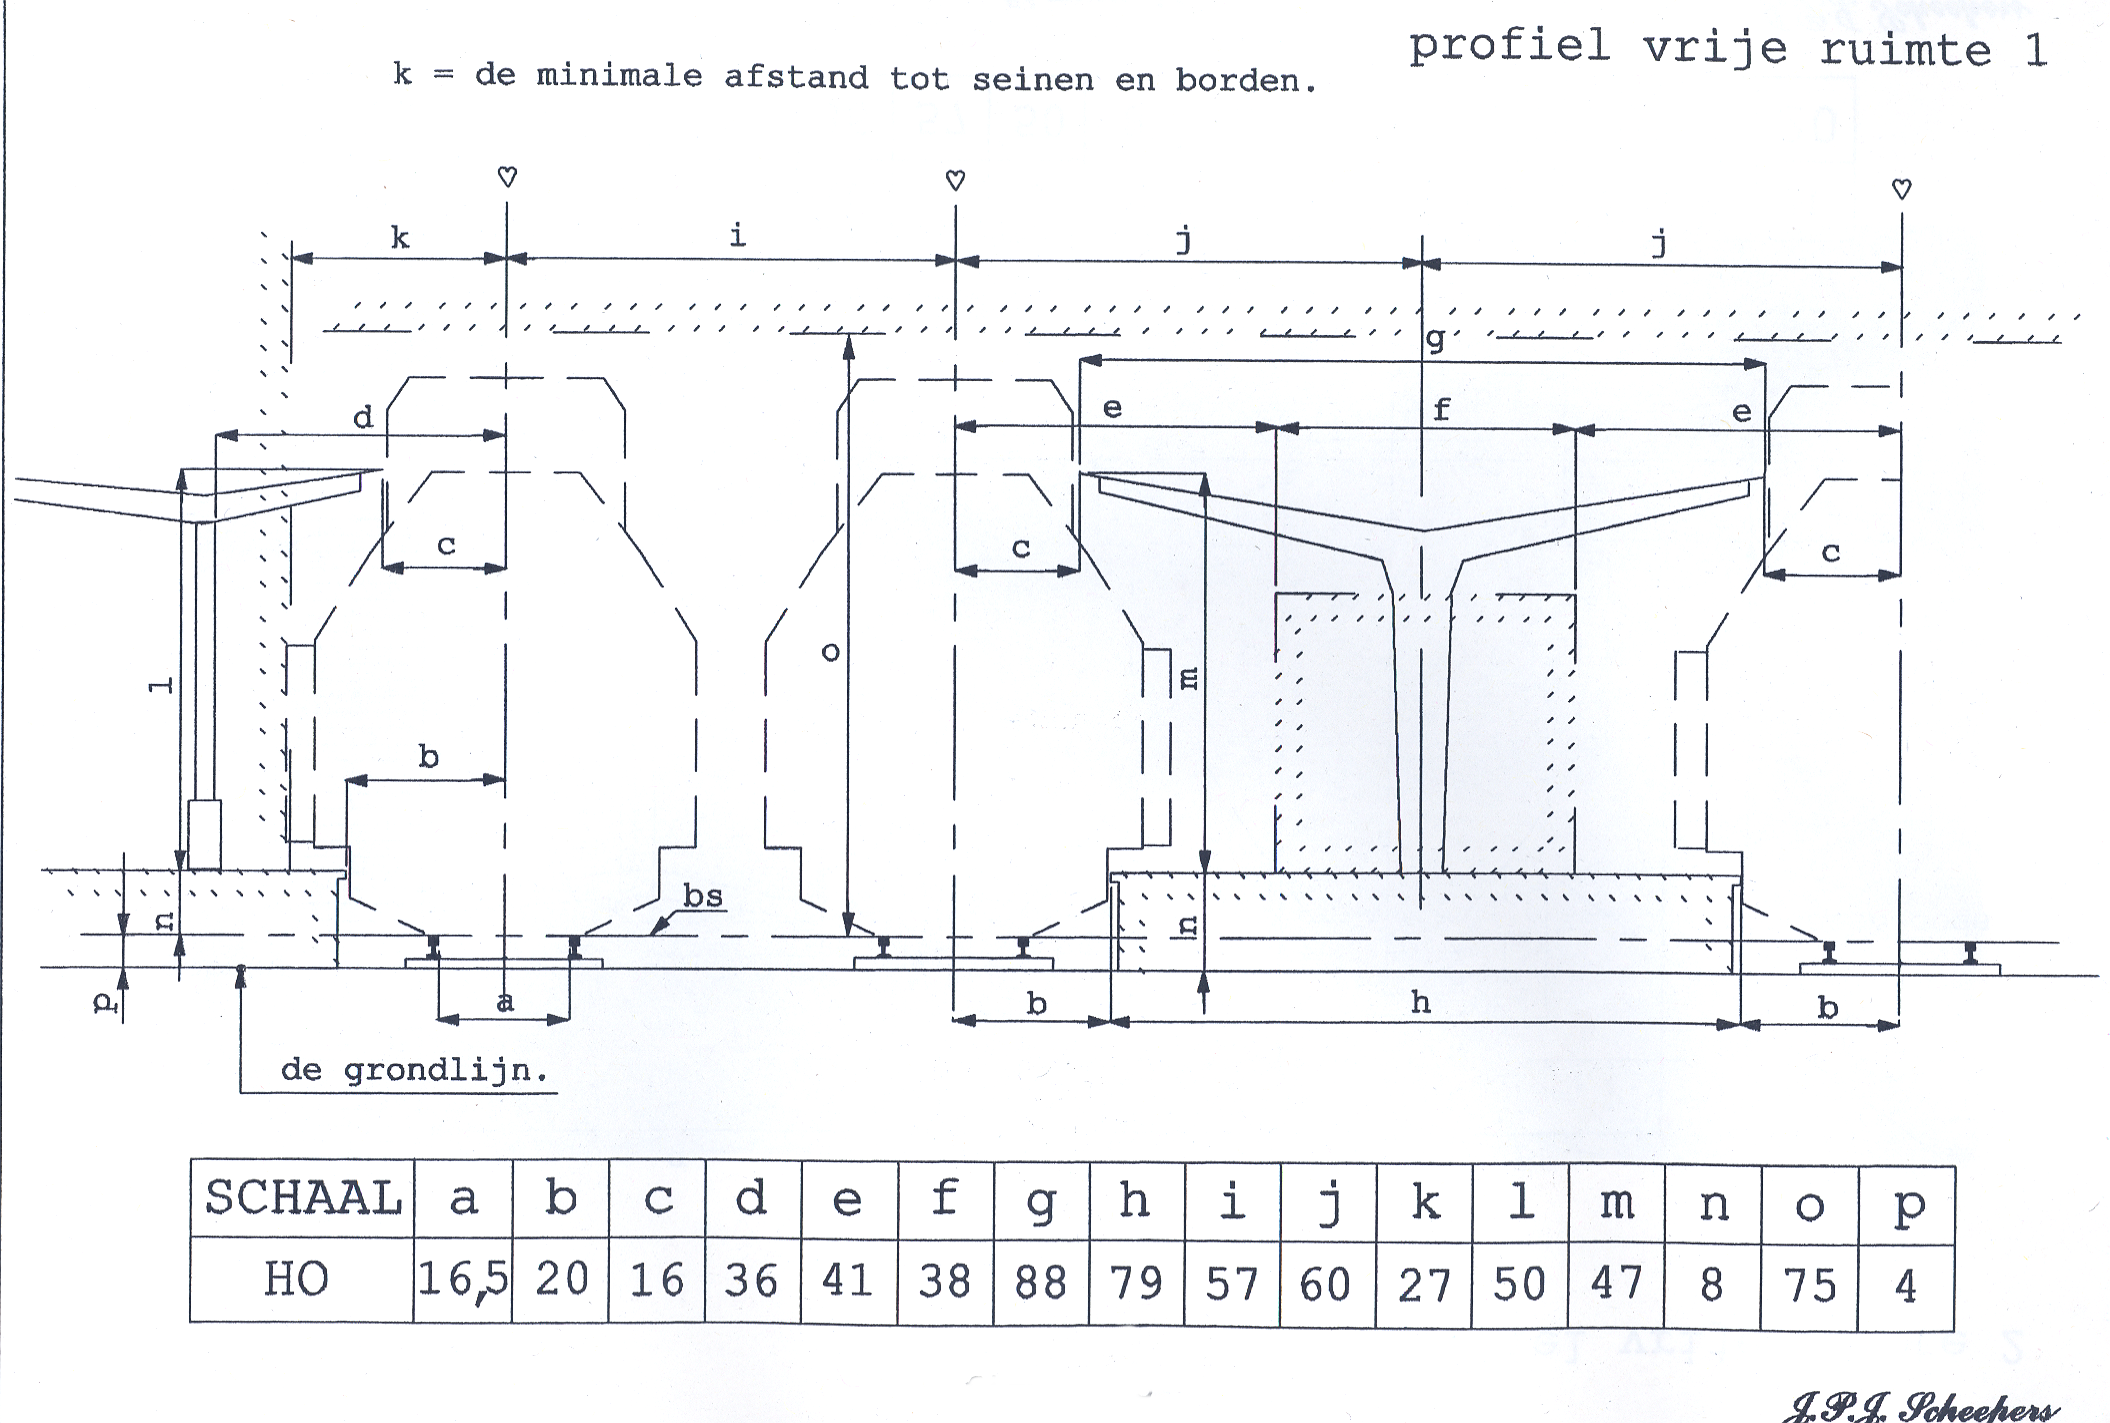
\includegraphics[scale=0.6]{images/rcu_figuur15}}
\end{figure}

\begin{figure}[!ht]
  \captionbox
  {Profiel vrije ruimte 2\label{figuur16}}
  {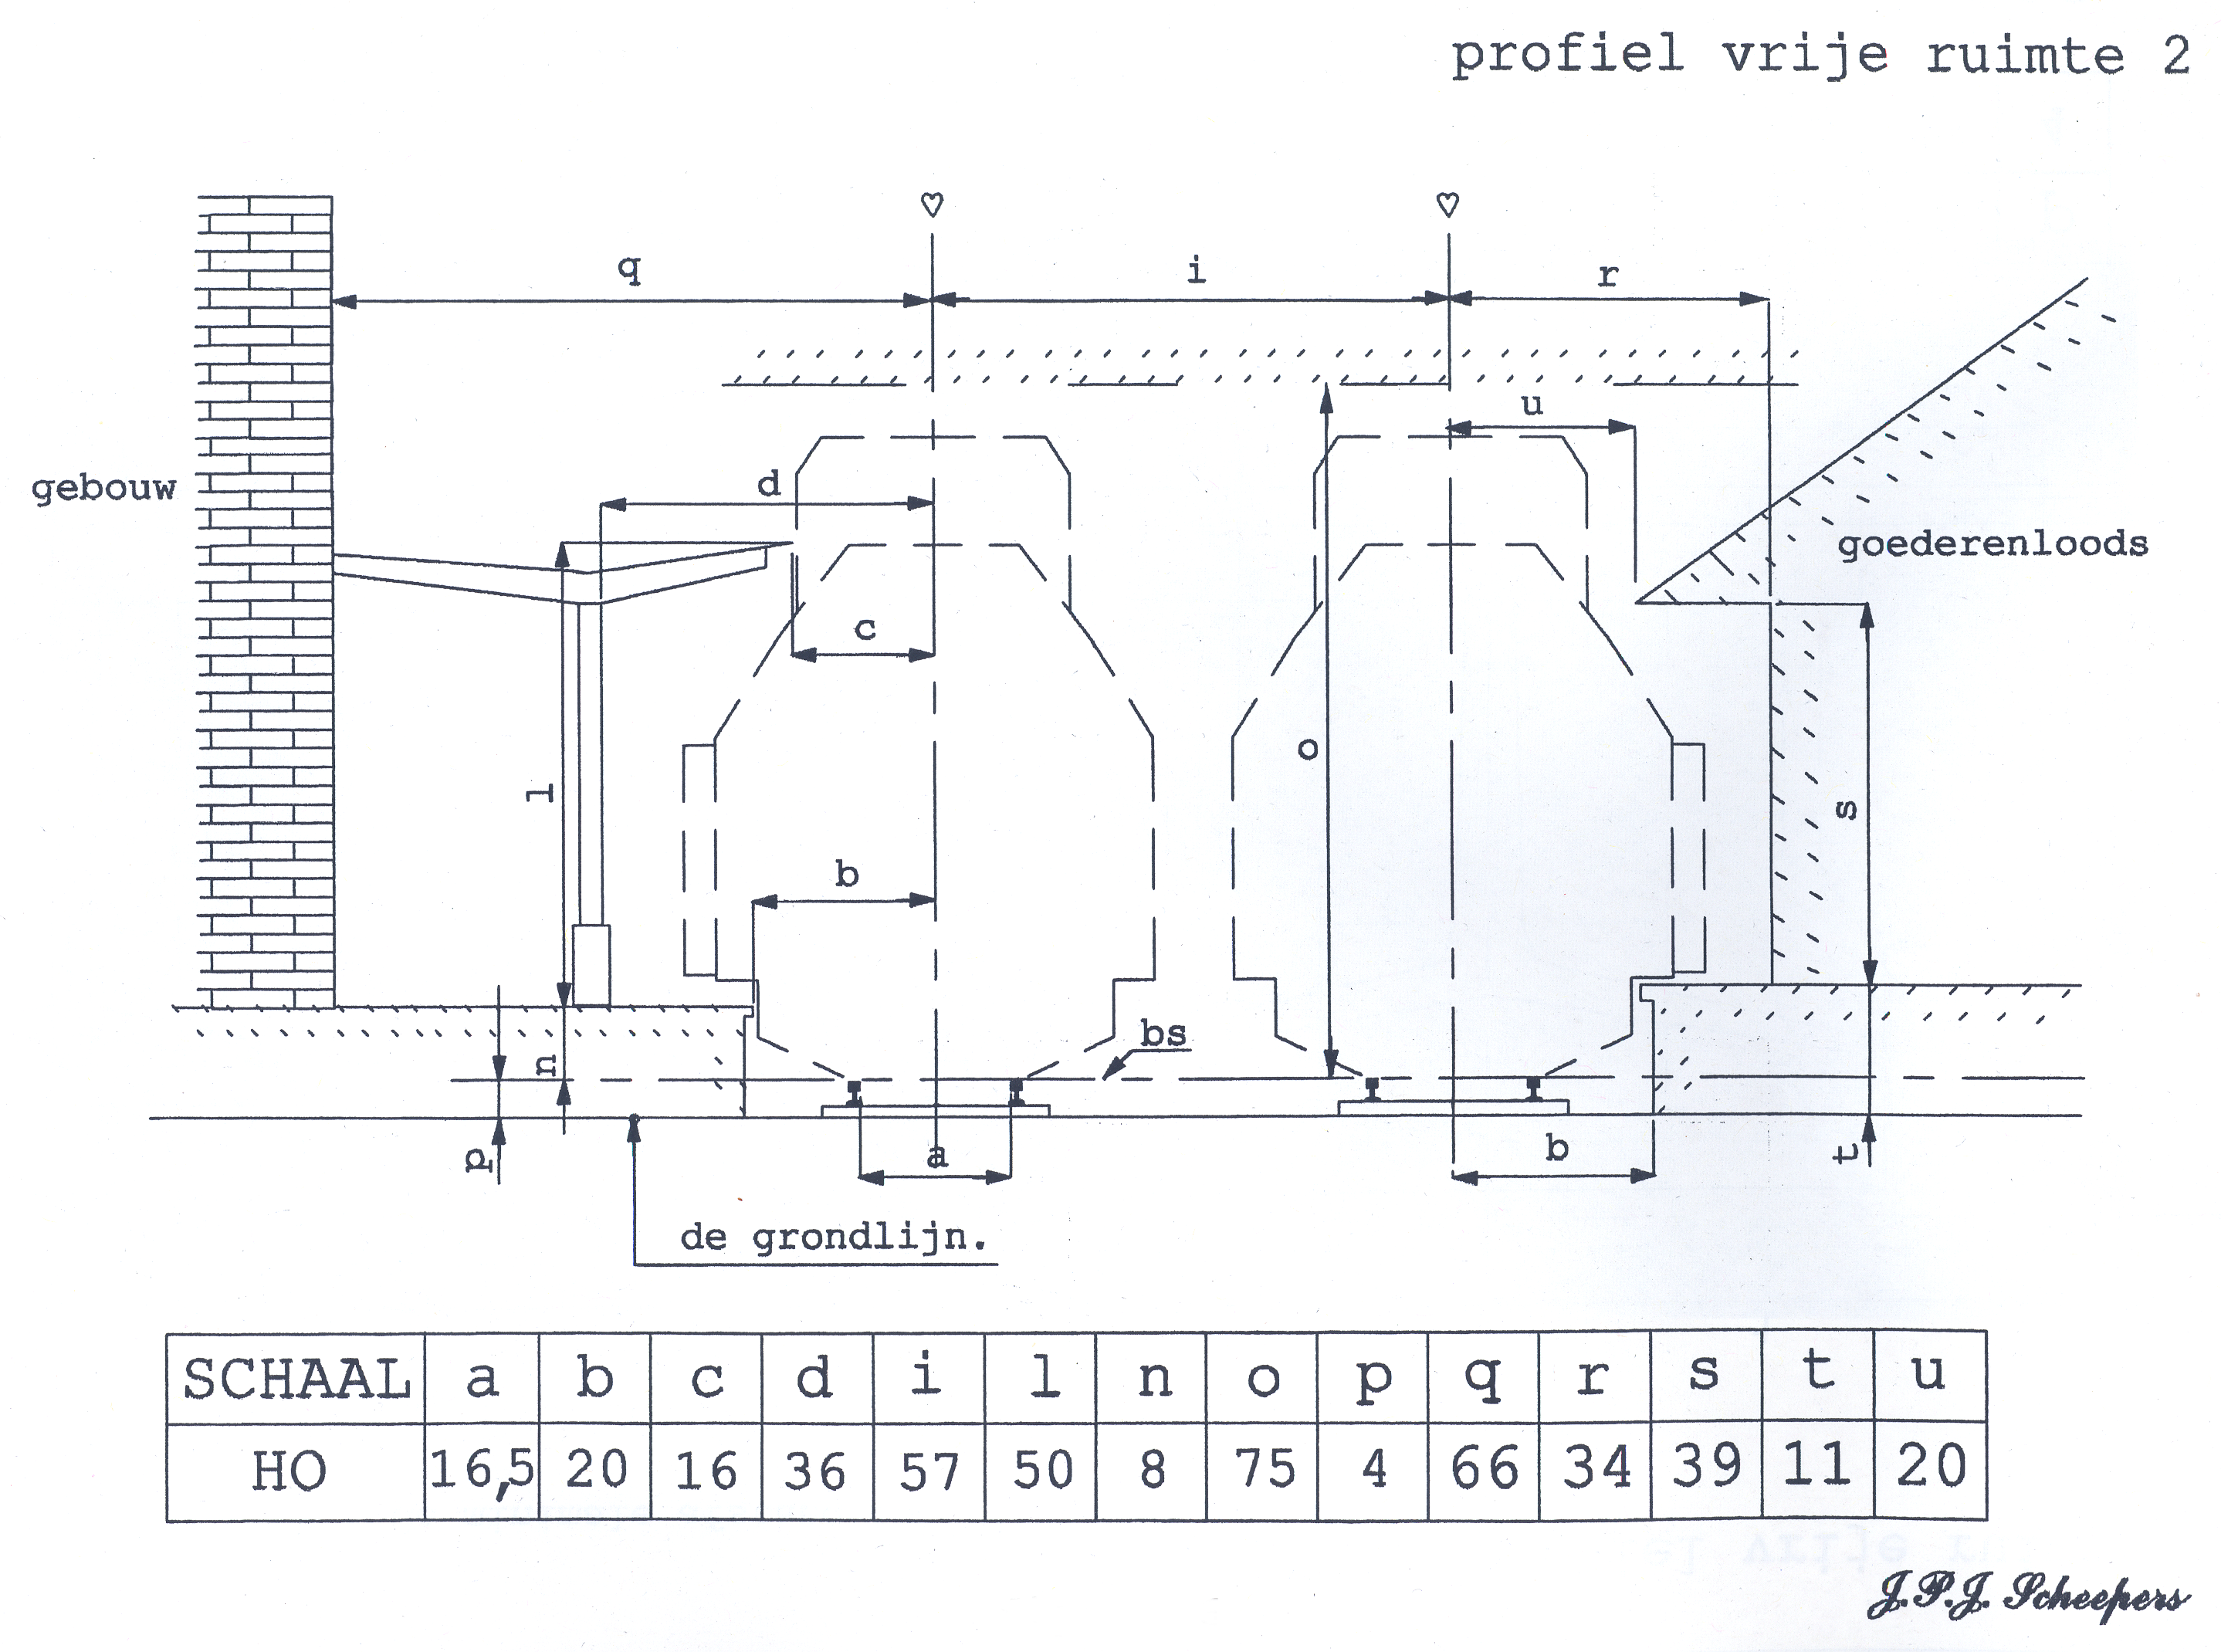
\includegraphics[scale=0.6]{images/rcu_figuur16}}
\end{figure}

In bogen, zowel op de vrije baan als bij gebogen perrons, is het raadzaam de vrije ruimte proefondervindelijk vast te stellen. De straal van de boog bepaalt namelijk hoever de rijtuigen overhangen in die boog.

\section{Optreden bij tentoonstellingen}

Om alles wat onder de baan wordt opgeborgen bij een tentoonstelling aan het oog van het publiek te onttrekken hangen er doeken rond de baan. Deze doeken worden opgehangen m.b.v. klittenband dat is bevestigd op latten die aan de baan worden vastgeschroefd met M5 schroeven. In de module zitten een aantal inslagmoeren bevestigd ter hoogte van iedere bovenleidingportaal. De lat is twee centimeter korter dan de module en 8 mm dik. De lat heeft een hoogte van 5 cm. In het midden zijn gaten geboord van 7 mm doornsnede. Om alle doeken op dezelfde hoogte te krijgen zijn de inslagmoeren 50 mm vanaf de onderkant van de module gemonteerd. Zie figuur \ref{figuur17}.

\begin{figure}[!ht]
  \captionbox
  {Positie klittenband t.b.v. doeken\label{figuur17}}
  {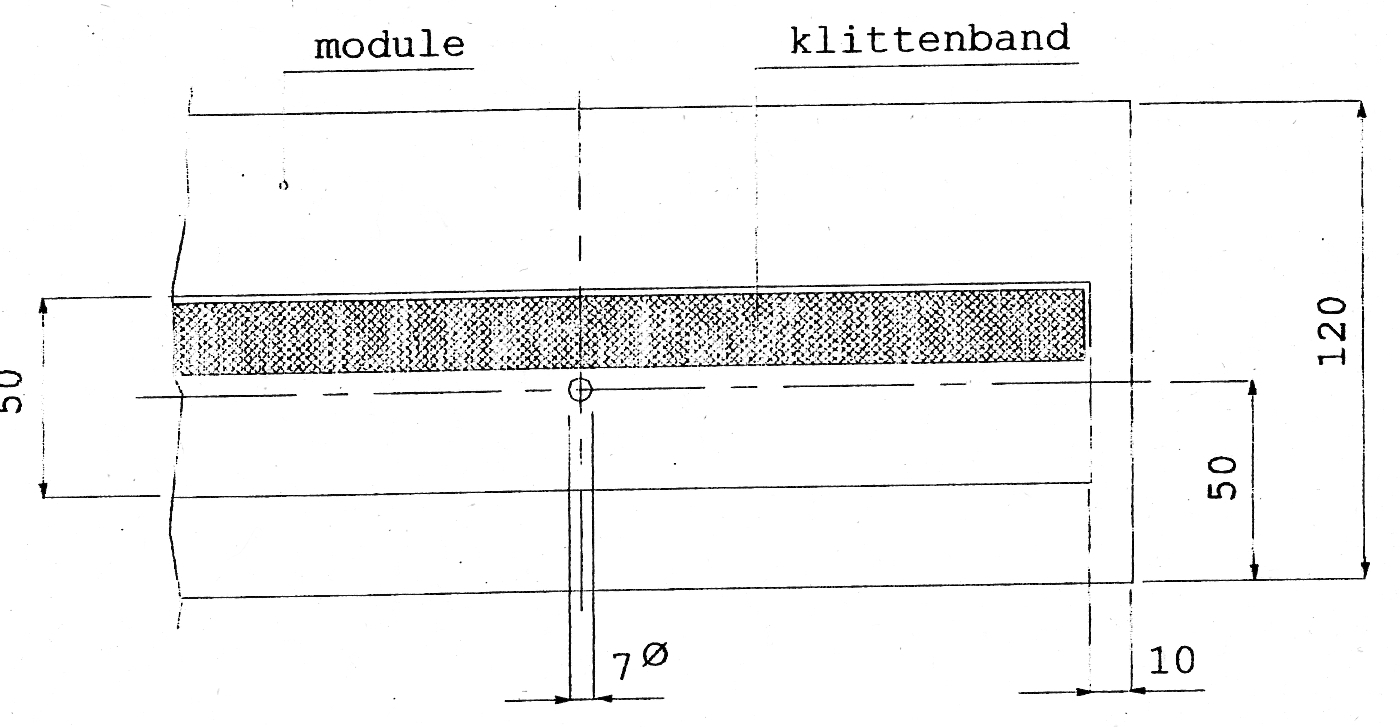
\includegraphics[scale=0.4]{images/rcu_figuur17}}
\end{figure}

Zie ook het boekje voor de regels tijdens beurzen, opendagen ect.

\chapter{Modules, boosters en bezetmelders}
\label{ch:electronica}
\section{Inleiding}

In het kader van de samenwerking van de H0-groepen binnen RailClub Utrecht maken we gebruik van een gemeenschappelijke baan voor 2- en 3-rail materiaal. Ook werken we met een simpel digitaal systeem , waarmee het mogelijk is om zowel het \marklin (Motorola) protocol aan te sturen als het DCC protocol.
Hierbij zijn voor de aansturing de volgende oplossingen gevonden:
\begin{itemize}
\item MDRRC-II zelfbouw centrale (Project Robert Evers): dit is een goedkope manier om een universele centrale te bouwen, waarbij gebruik wordt gemaakt van goedkope, via eBay verkrijgbare elektronica gecombineerd met zelfbouw interfaces (kosten: ca. \euro 25 voor de centrale, ca. \euro 15 voor de interface en voeding.)
\item RCU/BNL booster/hub: dit is een project van clublid Hans Kuijpers, waarbij met simpele, goedkope elektronica een booster gemaakt kan worden (kosten ca. \euro 10), die ook gebruikt kan worden voor het aansluiten van Roco (Multi)muizen.
\item Roco/Fleischmann Multimaus: deze populaire handregelaars zijn bij veel leden bekend, en er zijn in de groep een aantal beschikbaar. Ook de oudere types (Roco Maus, Maus 2) kunnen (beperkt) ingezet worden.
\end{itemize}

In dit hoofdstuk wordt uitgelegd hoe een en ander wordt aangesloten en bediend. Ook wordt alle informatie beschreven die nodig is om de RCU H0-modules aan elkaar te verbinden, zowel met detectie als zonder. Hierbij wordt uitgegaan van de nieuwe manier van aansluiten, middels Wieland stekkers voor de rijspanning en banaanstekkers voor de detectiestukken.

\section{Modules}
De Modules zijn gebaseerd op de voormalige 'M-track' modules, zoals deze in gebruik waren bij de \marklin groep. Zie voor de mechanische  en elektrische beschrijving hoofdstukken \ref{ch:modules} en \ref{ch:elektra}.

\subsection{Omschakelen basismodules}
Er zijn 2 soorten modules bij deze baan: 'basis' modules met alleen 2 sporen, zonder wissels of seinen, deze worden gewoon doorgelust, en 'seinenmodules', deze zijn voorzien van een of meerdere van de volgende zaken:

\begin{itemize}
\item detectiestukken met aansluitdoos (altijd)
\item seinen (optioneel)
\item wissels (optioneel)
\item modulebooster (optioneel)
\end{itemize}

Elke seinenmodule is voorzien van detectiestukken, deze worden middels banaanstekkers verbonden aan het bezetmelder aansluitblok.  In dit aansluitblok zit een blauwe kabel en een dubbele netwerkaansluitdoos. De regels voor rijden op 2- of 3-rails zijn als volgt:

\begin{itemize}
\item 2-rails: blauwe kabel in linker aansluiting van netwerkaansluitdoos, netwerkkabel in rechter aansluiting.
\item 3-rails: blauwe kabel los of in rechter aansluiting, netwerkkabel in linker aansluiting.
\end{itemize}

Het is ook mogelijk om zonder de aansluitdoos te rijden, dan kunnen alle detectiesecties aan elkaar worden doorverbonden. De manier van omschakelen wordt dan anders:

\begin{itemize}
\item 2-rail: verbind de detectiesecties met de rijspanning (rode aansluiting op aansluitblok)
\item 3-rail: verbind de detectiesecties met de massa (zwarte aansluiting op aansluitblok)
\end{itemize}

\subsection{Bezetmeldersecties}
De opzet van de bezetmeldersecties is als volgt:
er zijn 2 soorten modules:

\begin{enumerate}
\item basismodule (geen seinen en/of wissels, alle sporen doorlopend verbonden)
\item module met seinen (eventueel wissels), elk spoor voorzien van 2 gelijke secties
\end{enumerate}

Een blok bestaat uit 3 secties: een detectiesectie, een remsectie en een stopsectie. Aan het eind van elke stopsectie staat een sein. Hieruit volgt dan ook dat elk blok per richting minimaal bestaat uit 2 modules: een basismodule en een seinenmodule, zie figuur \ref{im:3secties}:

\begin{figure}[!ht]
  \captionbox
  {Opstelling blok enkele richting\label{im:3secties}}
  {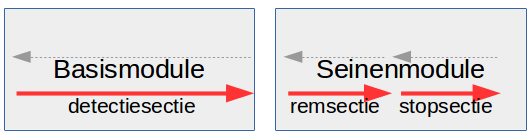
\includegraphics[scale=1.0]{images/rcu_3_secties}}
\end{figure}

In rood de beschreven secties: de basismodule bevat dus alleen een detectiesectie, de seinenmodule bevat de rem- en stopsectie. De gestippelde lijnen zijn de secties voor de andere richting.
Voor beide richtingen zijn dus minimaal 3 modules nodig: twee basismodules en een seinenmodule.
Elke module is met elkaar verbonden met een wielandstekker voor de (digitale) spanning. De detectiestukken zijn altijd de binnenste railstaven, en deze zijn verbonden aan de groene chassisdelen voor de banaanstekkers:
\begin{itemize}
\item Bij een \emph{basismodule} zijn deze chassisdelen per richting aan elkaar doorverbonden (een basismodule kent ten slotte maar 1 detectiestuk per rijrichting).
\item Bij een \emph{seinenmodule} zijn de 2 detectiestukken per richting apart verbonden.
\end{itemize}

\subsection{Aansluiting detectiestukken}
De secties worden middels banaanstekkers verbonden aan het bezetmelder aansluitblok (figuur \ref{im:rcu_bezetmelderblok}). 

\begin{figure}[!ht]
  \captionbox
  {Bezetmelder aansluitblok\label{im:rcu_bezetmelderblok}}
  {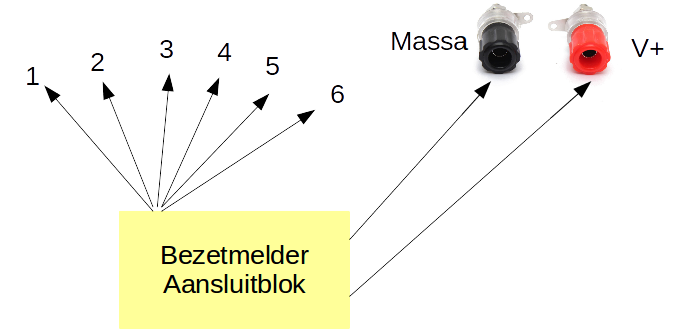
\includegraphics[scale=1.0]{images/rcu_bezetmelderblok}}
\end{figure}

Het bezetmelder aansluitblok is ook aangesloten aan de railspanningsaansluitingen van de vaste bekabeling van de module, op deze manier kan de stroom- en massadetectie worden gedetecteerd. Deze aansluitingen komen uit op 2 banaan chassisdelen op het aansluitblok, om eventueel de detectiesecties direct aan te sluiten (zie hoofdstuk 'Zonder bezetmeldersecties').
De aansluitingen van het aansluitblok worden aan de volgende secties aangesloten:

\begin{enumerate}
\item Detectiesectie achterste spoor
\item Remsectie achterste spoor
\item Stopsectie achterste spoor
\item Detectiesectie voorste spoor
\item Remsectie voorste spoor
\item Stopsectie voorste spoor
\end{enumerate}

Als er meerdere basismodules worden gebruikt als een sectie, moeten deze aan beide kanten aan elkaar worden doorverbonden middels doorverbindkabels (2 banaanstekkers groen), zie voorbeeld:

\subsection{Zonder bezetmeldersecties}
Bij het rijden zonder detectie kunnen alle detectiesecties aan elkaar worden doorverbonden. De manier van omschakelen wordt dan anders:

\begin{itemize}
\item 2-rail: verbind de detectiesecties met de rijspanning (rode aansluiting op aansluitblok)
\item 3-rail: verbind de detectiesecties met de massa (zwarte aansluiting op aansluitblok)
\end{itemize}

\section{Modulebooster/hub}

\begin{figure}[!ht]
  \captionbox
  {Bovenaanzicht modulebooster\label{modulebooster}}
  {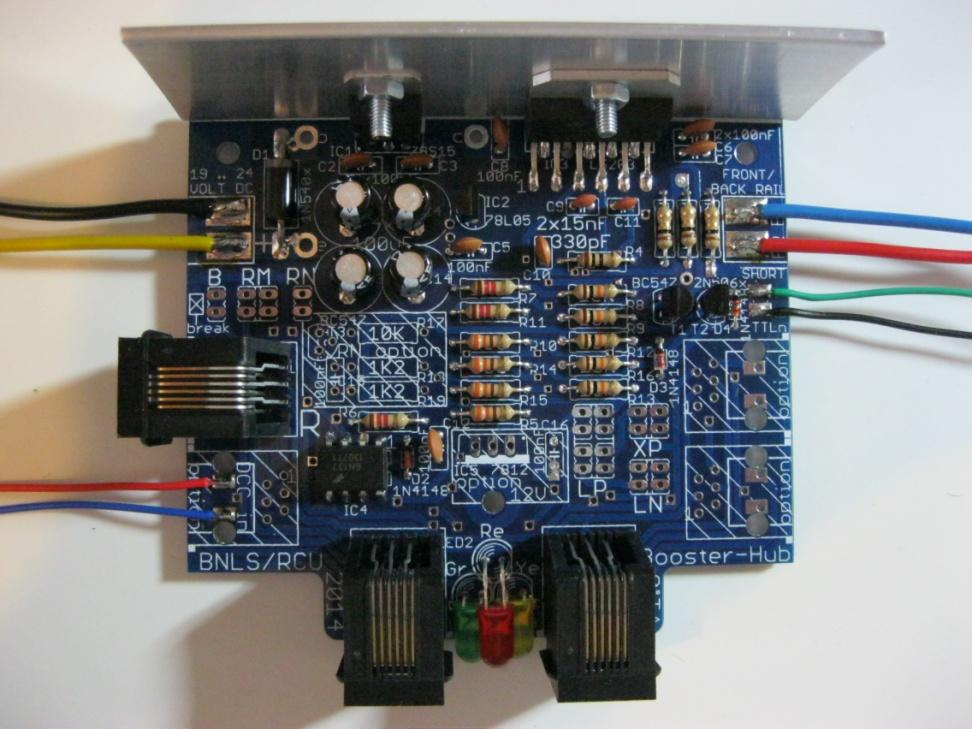
\includegraphics[scale=0.5]{images/rcu_foto3}\\}
\end{figure}

De boosters worden gemonteerd onder de 'basismodules', dit zijn modules die voorzien zijn van bezetmeldersecties en seinen. Elke booster heeft een eigen voeding (\marklin-voeding van 18V/2A) die vast wordt aangesloten onder de module. De voedingskabel hiervan moet dus bij de opbouw worden aangesloten op 230V.
Verder zitten nog aangesloten op de booster:
\begin{itemize}
\item een vast gemonteerde drukknop voor het resetten na een kortsluiting: na het oplossen van de kortsluiting (onderste ledje aan) kan de booster worden gereset door deze knop in te drukken (onderste ledje moet weer uit gaan).
\item aan de voorkant, gemonteerd op de zijkant van de module, 2 aansluitingen voor de Roco muizen.
\item 3 statusleds, met de volgende betekenis (van voren af gezien):\\

\begin{table}[!ht]
\centering
\label{my-label}
\begin{tabular}{l|l|l}
\cline{2-2}
                           & Voeding Aanwezig &                           \\ \hline
\multicolumn{1}{|l|}{Digitaal Signaal Aanwezig} &      & \multicolumn{1}{l|}{Kortsluiting gedetecteerd} \\ \cline{1-1} \cline{3-3} 
\end{tabular}
\end{table}

\item 2 RJ12 (XpressNet)aansluitingen aan de zijkant voor de XpressNet kabel van de centrale en naar de volgende module (aansluitingen zijn doorgelust)
\item een railuitgang die wordt aangesloten aan 2 banaanstekkers (rood voor signaal, zwart voor aarde).
\end{itemize}

Let op: je kunt dus een andere booster op de baan aansluiten, als je zorgt dat de modulebooster losgekoppeld is middels de banaanstekkers en de voeding.

\subsection{Gebruik meerdere boosters en boosterscheiding}
Bij gebruik van meerdere boosters in de baan (1 booster per basismodule), moeten deze van elkaar gescheiden worden, qua rijspanning. Hiervoor moet tussen 2 modules een 'boosterscheidingskabel' worden gemaakt, voorzien van 2 Wieland connectoren, met de tekst 'boosterscheiding (zie figuur \ref{im:boosterscheiding}). Het is voor de detectie niet relevant waar deze boosterscheiding komt.

\begin{figure}[!ht]
  \captionbox
  {Boosterscheidingskabel\label{im:boosterscheiding}}
  {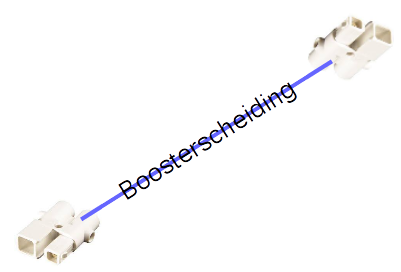
\includegraphics[scale=1.0]{images/rcu_boosterscheiding}}\\
\end{figure}

Als dit nog niet gebeurd is moet er maar 1 booster actief gemaakt worden, dus 1 booster aan 230V, en  de andere boosters niet aansluiten!

\chapter{Universele Centrale (DCC/Motorola)}
\label{ch:centrale}
De centrale bestaat uit een elektronicamodule met touchscreen en interface (zie bijlage \ref{ch:interface_centrale}). De centrale is inmiddels in een kastje ingebouwd, en ziet er als volgt uit (figuur \ref{centrale}):
\\

\begin{figure}[!ht]
  \captionbox
  {Bovenaanzicht MDRRC-II centrale\label{centrale}}
  {\includegraphics[scale=0.1]{images/rcu_foto1}}\\
\end{figure}

Bij het opstarten of resetten van de centrale zie je linksonder in het scherm de huidige configuratie (zie figuur \ref{rcu-foto4}):

\begin{figure}[!ht]
  \captionbox
  {Opstartscherm MDRRC-II centrale\label{rcu-foto4}}
  {\includegraphics[scale=0.6]{images/rcu_foto4}}\\
\end{figure}

\begin{enumerate}
\item PowerOff: geeft aan dat op dit moment de centrale geen signaal doorgeeft, door op de knop 'ON' te drukken op het touchscreen of op de kast (Stop/Go) kan de centrale worden ingeschakeld.
\item Locs : 52 [nr]: Hoeveel locs er zijn gedefinieerd, zowel DCC als MM (Motorola), en hierna hoeveel daarvan als MM zijn gedefinieerd.
\item S88  : 32 [nr] Freq : 10000 :Hoeveel S88 terugmeldmodules zijn geconfigureerd, en wat de uitleesfrequentie is
\item Xnet : On  I2C : On : Of XpressNet (Xnet) aan staat, en of de andere interface aan staat (\isqc, wordt niet gebruikt)
\end{enumerate}

\section{Aansluiting Centrale aan booster(s)}
De centrale wordt middels de XpressNet kabels aan de boosters aangesloten, de boosters worden hier onderling ook mee aangesloten. De (Multi)muizen moeten dan aan de boosters worden aangesloten. Het maakt niet uit waar in de keten de centrale wordt aangesloten, zie figuur \ref{im:aansluiten_booster}.

\begin{figure}[!ht]
  \captionbox
  {Aansluiten Centrale en Boosters\label{im:aansluiten_booster}}
  {\includegraphics[scale=0.5]{images/rcu_schema1}\\}
\end{figure}

De achterkant van de centrale ziet er als volgt uit (figuur \ref{centrale_achter}):\\

\begin{figure}[!ht]
  \captionbox
  {Achteraanzicht MDRRC-II centrale\label{centrale_achter}}
  {\includegraphics[scale=0.3]{images/rcu_foto5}\\}
\end{figure}

Er zijn dus 3 aansluitingen:\\

\begin{tabular}{|l |p{10cm}|}
\hline
USB&voor aansluiting aan een computer, voor configuratie of sturen middels Koploper, Itrain, Rocrail, etc\\
\hline
S88&Hier worden de terugmeldmodules op aangesloten. Hiervoor moet de configuratie van de centrale overeenstemmen met het aantal modules wat er op wordt aangesloten, dit is geen plug \& play!\\
\hline
X(press)net/Booster&Hier worden de boosters op aangesloten, via een 6-aderige platte (telefoon)kabel. Sluit hier geen MultiMaus op aan, je kunt de centrale en/of Multimaus hiermee beschadigen!\\
\hline
\end{tabular}\\

\section{Rijden met Locs}
Default staat de centrale ingesteld op een bepaald protocol, dus \`{o}f DCC \`{o}f Motorola; dit betekent niet dat er geen andere locs aangestuurd kunnen worden, alleen welk formaat standaard is als er een nieuwe loc bijkomt. Om dit te wijzigen moet je een parameter van de centrale wijzigen, zie bijlage \ref{ch:config}.\\
Er zijn meerdere manieren om locs bekend te maken in de centrale, een van de makkelijkste manieren is via de 'loc bibliotheek' van de Roco Multimaus:
\begin{enumerate}
\item Zorg dat de loc in de Multimaus is aangemaakt met naam en adres (andere parameters zijn niet belangrijk).
\item Zet de MDRRC-II centrale op 'Receive Loc Library': 
\subitem Reset de centrale
\subitem Druk op 'SET'
\subitem Druk op 'LL'
\subitem Druk op 'RLL'
\item Zet de Multimaus op 'Send' (Menu Loc)
\item Nu worden alle locs uit de Multimaus locbibliotheek ingelezen, op het touchscreen van de centrale worden alleen de nog niet bekende getoond.
\end{enumerate}

Al deze locs worden nu dus aangestuurd met het 'default' protocol, je kunt het type wel wijzigen per lokadres.\\
Met het Motorola protocol kun je ook \marklin 'Delta' decoders aansturen, de relatie tussen de 'Delta' adressen en de Motorola adressen is als volgt:\\

\begin{table}[!ht]
\begin{tabular}{|l|l|}
\hline
Delta adres&Motorola Adres\\
\hline
1&78\\
\hline
2&72\\
\hline
3&60\\
\hline
4&24\\
\hline
5&80\\
\hline
\end{tabular}
\caption{\marklin \ Delta adressen}
\end{table}

Zie ook \url{http://encyclopedie.beneluxspoor.net/index.php/Het_Motorola_protocol}

\subsubsection{Toevoegen Loc}
Om een loc toe te voegen, ga je als volgt te werk:

\begin{enumerate}
\item Zet de MDRRC-II centrale op 'Add Loc': 
\subitem Reset de centrale
\subitem Druk op 'SET'
\subitem Druk op 'LOC'
\subitem Druk op 'ADD'
\item Type nu op het numerieke cijferblok het adres in van de loc, als je verkeerd typte springt het nummer na 4 cijfers weer op 0.
\item Druk op 'MM' om een loc met een Motorola-decoder toe te voegen, of op 'DCC' om een loc met een DCC-decoder toe te voegen
\end{enumerate}

Als de loc al in het systeem staat zie je een foutmelding:
 'Loc XX already present!!!'
je kunt hem dan eventueel verwijderen of wijzigen van type. Als het toevoegen succesvol is, zie je de melding: 'Loc XX added decoder type \textless type\textgreater ', 
waarbij \textless type\textgreater  MM of DCC is.
\subsubsection{Verwijderen loc}
Om een loc te verwijderen, ga je als volgt te werk:
\begin{enumerate}
\item Zet de MDRRC-II centrale op 'Delete Loc': 
\subitem Reset de centrale
\subitem Druk op 'SET'
\subitem Druk op 'LOC'
\subitem Druk op 'DEL'
\item Selecteer nu met + en - de gewenste loc in de centrale.
\item Druk op 'DEL' om de loc te verwijderen uit de centrale. Je krijgt nu op het scherm de melding:
Deleted Loc: XX
\item De loc is nu verwijderd uit het systeem, de centrale springt nu naar de volgende loc, je kunt nu verder met stap 2, of weer terug naar het Locmenu met de optie 'Loc'.
\end{enumerate}

\subsubsection{Wisselen Decodertype (vanaf softwareversie 3.6.1)}
Het is mogelijk om het type van de locomotief te veranderen: van DCC naar MM en omgekeerd.
\begin{enumerate}
\item Zet de MDRRC-II centrale op 'Change Loc Decoder Type': 
\subitem Reset de centrale
\subitem Druk op 'SET'
\subitem Druk op 'LOC'
\subitem Druk op 'CHD'
\item Selecteer nu met + en - de gewenste loc in de centrale.
\item Druk op 'CHD' om het Decodertype te wisselen, je ziet nu op het scherm wat de wijziging is.
\end{enumerate}

\section{Sturen van seinen en Wissels}
Net als bij locs is er ook een default protocol voor het aansturen van stationaire decoders (sein/wisseldecoders); dit staat standaard op 'Motorola'.
Per decoderadres kan dit omgewisseld worden:

\begin{enumerate}
\item Zet de MDRRC-II centrale op 'Change Turnout Decoder Type': 
\subitem Reset de MDRRC-II centrale
\subitem Druk op 'ON'
\subitem Druk op 'OPT'
\subitem Druk op 'SET'
\item Kies nu op de Multimaus het adres van de decoder die omgewisseld moet worden
\item Door nu deze decoder aan te sturen, wordt hij omgewisseld van MM naar DCC en weer omgekeerd, dit kun je volgen op het touchscreen.
\end{enumerate}

\appendix

\chapter{Testen Modules}
\label{ch:testen}
Voor het testen van de modules is een testkastje gemaakt, die controleert of de aansluitingen van de module nog correct zijn.

\begin{figure}[!ht]
  \captionbox
  {Testkastje Modules\label{im:testkastje}}
  {\includegraphics[scale=1.0]{images/rcu_foto2}\\}
\end{figure}

Dit testkastje bevat een batterij, een omschakelaar (enkel of dubbel), 3 leds en 3 drukknoppen, en is bedoeld voor het testen per railaansluiting (links-midden-rechts) op kortsluiting, en of de aansluitingen contact hebben met het rollend materiaal wat erop staat. 
Het is voorzien van 2 sets kabels met elk een wielandstekker en een banaanstekker, voor de linkerkant (aansluiting 1) en de rechterkant (aansluiting 2) van de baan.

\section{Zelftest: controle testkastje}
\begin{itemize}
\item koppel het kastje helemaal los (Wieland stekkers en banaanstekkers los aan beide kanten) 
\item stel het testkastje in op 'enkelzijdig' 
\item Verwacht resultaat:\\
\\
\begin{tabular}{|l|l|l|l|}
\hline
Drukknop&Led 1&Led 2&Led 3\\
\hline
1 (Signaal)&Aan&Uit&Uit\\
\hline
2 (Massa)&Uit&Aan&Uit\\
\hline
3 (Detectie)&Uit&Uit&Aan\\
\hline
\end{tabular}

Mogelijke oorzaken als resultaat afwijkt:\\
\begin{tabular}{|p{8cm}|p{6cm}|}
\hline
geen enkele led gaat branden bij indrukken drukknop:&batterij testkastje op of niet goed aangesloten\\
\hline
meerdere leds gaan aan bij indrukken 1 drukknop:&kortsluiting in het kastje\\
\hline
\end{tabular}\\

\item stel het testkastje in op 'dubbelzijdig' 
\item Verwacht resultaat:\\
\\
\begin{tabular}{|l|l|l|l|}
\hline
Drukknop&Led 1&Led 2&Led 3\\
\hline
1 (Signaal)&Uit&Uit&Uit\\
\hline
2 (Massa)&Uit&Uit&Uit\\
\hline
3 (Detectie)&Uit&Uit&Uit\\
\hline
\end{tabular}

\item Mogelijke oorzaken als resultaat afwijkt:\\
\begin{tabular}{|p{8cm}|p{6cm}|}
\hline
Een of meerdere leds gaan aan bij indrukken 1 drukknop:&kortsluiting in het kastje\\
\hline
\end{tabular}\\

\item koppel de kabels van het kastje aan elkaar (Wieland stekkers + banaanstekker).
\item stel het testkastje in op 'dubbelzijdig' 
\item Verwacht resultaat:\\
\\
\begin{tabular}{|l|l|l|l|}
\hline
Drukknop&Led 1&Led 2&Led 3\\
\hline
1 (Signaal)&Aan&Uit&Uit\\
\hline
2 (Massa)&Uit&Aan&Uit\\
\hline
3 (Detectie)&Uit&Uit&Aan\\
\hline
\end{tabular}

\item Mogelijke oorzaken als resultaat afwijkt:\\
\begin{tabular}{|p{8cm}|p{6cm}|}
\hline
meerdere leds gaan aan bij indrukken 1 drukknop&kortsluiting in het kastje of kabel\\
\hline
Geen enkele led gaat aan&batterij op of kabels defect\\
\hline
\end{tabular}

\end{itemize}

\section{kortsluittest op module zonder rijdend materieel - enkel}

\begin{figure}[!ht]
  \captionbox
  {Kortsluittest enkel\label{im:test_enkel}}
  {\includegraphics[scale=0.8]{images/rcu_test_enkel}\\}
\end{figure}

\begin{itemize}
\item koppel de module helemaal los (Wieland stekkers en banaanstekkers los aan beide kanten) 
\item Zorg dat er geen rollend materiaal op de module staat
\item koppel het testkastje aan de linkerkant van de module: 1 x Wieland stekkers plus de banaanstekker van het spoor wat je wil testen. 

\item stel het testkastje in op 'enkel' 
\item Verwacht resultaat:
\\
\begin{tabular}{|l|l|l|l|}
\hline
Drukknop&Led 1&Led 2&Led 3\\
\hline
1 (Signaal)&Aan&Uit&Uit\\
\hline
2 (Massa)&Uit&Aan&Uit\\
\hline
3 (Detectie)&Uit&Uit&Aan\\
\hline
\end{tabular}

\item Mogelijke oorzaken als resultaat afwijkt:\\
\begin{tabular}{|p{8cm}|p{6cm}|}
\hline
geen enkele led gaat branden bij indrukken drukknop&batterij testkastje op of niet goed aangesloten\\
\hline
meerdere leds gaan aan bij indrukken 1 drukknop&kortsluiting tussen de sporen\\
\hline
\end{tabular}

\end{itemize}

\section{kortsluittest op module zonder rijdend materieel - dubbel}

\begin{figure}[!ht]
  \captionbox
  {Kortsluittest dubbel\label{im:test_dubbel}}
  {\includegraphics[scale=0.8]{images/rcu_test_dubbel}\\}
\end{figure}

\begin{itemize}
\item koppel de module helemaal los (Wieland stekkers en banaanstekkers los aan beide kanten)
\item Zorg dat er geen rollend materiaal op de module staat
\item koppel het testkastje aan beide kanten van de module:
\subitem 1 x Wieland stekkers van de linkerkant plus de banaanstekker van het spoor wat je wil testen aan de kabels voor aansluiting 1,
\subitem 1 x Wieland stekkers van de rechterkant plus de banaanstekker van het spoor wat je wil testen aan de kabels voor aansluiting 2

\item stel het testkastje in op 'dubbel' 
\item Verwacht resultaat:\\

\begin{tabular}{|l|l|l|l|}
\hline
Drukknop&Led 1&Led 2&Led 3\\
\hline
1 (Signaal)&Aan&Uit&Uit\\
\hline
2 (Massa)&Uit&Aan&Uit\\
\hline
3 (Detectie)&Uit&Uit&Aan (*)\\
\hline
\end{tabular}

	* : aan bij standaardmodule, uit bij seinenmodule
\item Mogelijke oorzaken als resultaat afwijkt:\\
\begin{tabular}{|p{8cm}|p{6cm}|}
\hline
geen enkele led gaat branden bij indrukken drukknop&batterij testkastje op of niet goed aangesloten, kabel niet goed aangesloten aan een van beide kanten of geen verbinding tussen linker- en rechterzijde module (*): dit is correct voor drukknop 3 als het een seinenmodule betreft!\\
\hline
meerdere leds gaan aan bij indrukken 1 drukknop&kortsluiting tussen de sporen\\
\hline
\end{tabular}

\end{itemize}

\section{verbindingstest op module met rijdend materieel (3-rail)}

\begin{figure}[!ht]
  \captionbox
  {Kortsluittest dubbel met materieel\label{im:test_dubbel_met}}
  {\includegraphics[scale=0.8]{images/rcu_test_dubbel_met}\\}
\end{figure}

\begin{itemize}
\item koppel de module helemaal los (Wieland stekkers en banaanstekkers los aan beide kanten) 
\item Zet rollend materiaal op de baan: een loc of een wagen met verlichting waarvan zeker is dat deze goed is.
\item koppel het testkastje aan de linkerkant van de module: 1 x Wieland stekkers plus de banaanstekker van het spoor wat je wil testen.

\item stel het testkastje in op 'enkelzijdig' 

\item Verwacht resultaat:

\begin{tabular}{|l|l|l|l|}
\hline
Drukknop&Led 1&Led 2&Led 3\\
\hline
1 (Signaal)&Aan&Brandt zwak&Brandt zwak\\
\hline
2 (Massa)&Brandt zwak&Aan&Aan\\
\hline
3 (Detectie)&Brandt zwak&Aan&Aan\\
\hline
\end{tabular}

\item Mogelijke oorzaken als resultaat afwijkt:

\begin{tabular}{|p{8cm}|p{6cm}|}
\hline
geen enkele led gaat branden bij indrukken drukknop&batterij testkastje op of niet goed aangesloten\\
\hline
De andere leds branden helemaal niet bij indrukken drukknop 1&materiaal maakt geen contact met de baan via de sleper en puko's\\
\hline
Bij indrukken drukknop 2 brandt led 3 niet (of omgekeerd)&wielen zijn ge\"{i}soleerd (geen verbinding van railstaven via wielen, materiaal staat op ander gedeelte van seinenmodule\\
\hline
Bij indrukken drukknop 2 of 3 brandt led 1 helemaal niet&materiaal maakt geen contact met de baan via de sleper en puko's\\
\hline
\end{tabular}

\end{itemize}

\section{verbindingstest op module met rijdend materieel (2-rail)}

\begin{figure}[!ht]
  \captionbox
  {Kortsluittest dubbel met materieel 2-rail\label{im:test_dubbel_met_2rail}}
  {\includegraphics[scale=0.8]{images/rcu_test_dubbel_met_2rail}\\}
\end{figure}

\begin{itemize}
\item koppel de module helemaal los (Wieland stekkers en banaanstekkers los aan beide kanten) 
\item Zet rollend materiaal op de baan: een loc of een wagen met verlichting waarvan zeker is dat deze goed is.
koppel het testkastje aan de linkerkant van de module: 1 x Wieland stekkers plus de banaanstekker van het spoor wat je wil testen.

\item stel het testkastje in op 'enkelzijdig' 

\item Verwacht resultaat:

\begin{tabular}{|l|l|l|l|}
\hline
Drukknop&Led 1&Led 2&Led 3\\
\hline
1 (Signaal)&Aan&Uit&Uit\\
\hline
2 (Massa)&Uit&Aan&Brandt zwak\\
\hline
3 (Detectie)&Uit&Brandt zwak&Aan\\
\hline
\end{tabular}

\item Mogelijke oorzaken als resultaat afwijkt:

\begin{tabular}{|p{8cm}|p{6cm}|}
\hline
geen enkele led gaat branden bij indrukken drukknop&batterij testkastje op of niet goed aangesloten\\
\hline
De andere leds branden bij indrukken drukknop 1&materiaal maakt contact met de baan via een sleper en puko's\\
\hline
Bij indrukken drukknop 2 brandt led 3 helemaal niet (of omgekeerd)&materiaal maakt geen (goed) contact met railstaven, of materiaal staat op ander gedeelte van seinenmodule\\
\hline
Bij indrukken drukknop 2 of 3 brandt led 1&materiaal maakt contact met de baan via een sleper en puko's\\
\hline
\end{tabular}

\end{itemize}

\chapter{Opbouw detectie aansluitblok}
\label{ch:detection}

Op dit blok bevinden zich de volgende componenten:
\begin{enumerate}
\item 8-voudige stroomdetectieprint.
\item dubbel RJ45 aansluitblok.
\item 6-voudige kroonsteen met kabels (1 meter) met groene banaanstekkers.
\item 2 x banaan chassisdeel voor rijspanning (rood) en massa (zwart).
\end{enumerate}

Op het dubbele RJ45-aansluitblok zijn aan de linker connector de detectiestukken aangesloten middels de kroonsteen met kabels en groene banaanstekkers, en aan de rechter connector de uitgangen van de stroomdetectieprint (alleen 1 t/m 6). Hierbij geldt de volgende normering:\\

\begin{tabular}{|l|p{10cm}|}
\hline
1&Detectiesectie achterste spoor\\
\hline
2&Remsectie achterste spoor\\
\hline
3&Stopsectie achterste spoor\\
\hline
4&Detectiesectie voorste spoor\\
\hline
5&Remsectie voorste spoor\\
\hline
6&Stopsectie voorste spoor\\
\hline
7&Massa (met sperdiode)\\
\hline
8&Rijspanning\\
\hline
\end{tabular}

\chapter{Beschrijving Interfaceprint MDRRC-II Centrale}
\label{ch:interface_centrale}

De centrale wordt middels een interfaceprint (figuur \ref{im:interface}) aangesloten aan de buitenwereld, hierin zitten de volgende hulpschakelingen:

\begin{itemize}
\item Voeding voor +5 en +12 volt (ingang is 12 volt 2A gelijkspanning)
\item USB-interface met 'type B' (printer) aansluiting
\item Interface naar XpressNet + DCC, voor (Multi)muizen en booster
\item Interface naar S88, voor terugmeldschakelingen
\item Interface naar draaiknop, voor handbediening locs
\end{itemize}

\begin{figure}[!ht]
  \captionbox
  {Schema MDRRC-II interface\label{im:interface}}
  {\includegraphics[scale=0.5]{images/rcu_schema2}\\}
\end{figure}

De interface is voorzien van een aparte 12 volt-voeding, en bevat dan dus de volgende aansluitingen:
\begin{itemize}
\item Booster/Hub/XpressNet: dit is een 6-polige kabel met RJ12 aansluitingen, deze loopt van de centrale naar de eerste modulebooster en wordt van daaruit doorgelust naar eventuele volgende moduleboosters.
\item S88n/Terugmelderaansluitingen (op dit moment niet gebruikt): dit zijn 8-polige netwerkkabels (RJ45/UTP), die per groep van 6 railsecties de bezetmeldingen aan de centrale doorgeven.
\item USB: middels een printerkabel (USB A-B kabel) wordt de centrale aan een PC aangesloten.
\end{itemize}

De centrale is voor de bediening van de baan verder niet nodig en kan op een plek buiten de baan worden neergezet (afhankelijk van de lengte van de kabels).
De werking van de centrale is afhankelijk van de gebruikte softwareversie, op dit moment is dat 3.8.2.
De vier knoppen onder het touchscreen hebben ook een functie, hoewel er op dit moment maar 2 worden gebruikt:

\begin{enumerate}
\item De knop helemaal links schakelt tussen 'On' en 'Off', kan dus gebruikt worden als een noodstop; deze knop is ook op de interfaceprint beschikbaar, en kan dus apart worden aangesloten.
\item De knop helemaal rechtsonder reset de centrale.
\end{enumerate}

\chapter{Programmeerschakeling Centrale}

Hoewel het voor het rijden met op de modulebaan niet nodig is, is het mogelijk om de centrale te voorzien van een uitbreiding zodat ook (DCC-)loks kunnen worden geprogrammeerd.

\begin{figure}[!ht]
  \captionbox
  {Terugmeldschakeling centrale}
  {\includegraphics[scale=0.7]{images/rcu-MDRRCII-ack}}
\end{figure}

\begin{itemize}
\item Weerstand 39 Ohm
\item Weerstand 680 Ohm
\item Weerstand 47kOhm
\item Diode 1N4004
\item Optocoupler PC814
\item Condensator 33nF
\end{itemize}

\chapter{Afmetingen gebruikte kast voor centrale}

Dit zijn de boormaten voor het inbouwen van de centrale met interfaceprint in een lessenaarkast (TEKO TK363G).

\begin{figure}[!ht]
  \captionbox
  {Boormaten lessenaarkastje (Teko TK363G)}
  {\includegraphics[scale=0.7]{images/inbouwmaten_centralekast}}
\end{figure}

\chapter{Terugmelderaansluitingen}
\label{ch:terugmeldingen}
Aan de centrale kun je terugmelders aansluiten van het type S88. Dit gaat middels de zogenaamde S88N-norm, die gebruik maakt van Rj45 (UTP)-stekkers, zoals ze gebruikt worden voor computernetwerken. Deze kabels zijn makkelijk te krijgen in diverse lengtes, en goedkoop.
Een eigenschap van S88 is dat het een 'keten' is van modules: de eerste module wordt verbonden met de tweede, de tweede met de derde, et cetera. De laatste module gaat naar de centrale. Een gevolg hiervan is dat de centrale moet weten hoe lang de keten is. Hierbij moet ook nog rekening worden gehouden met de grootte van een module. De centrale kent standaard 16-voudige modules, en moet dan ook worden ingesteld met het aantal van deze modules.
Dit gaat als volgt: 
\begin{enumerate}
\item Verbind de centrale met een computer middels USB
\item Open een terminalprogramma
\item Zet de centrale in configuratiemodus: 
\item Reset de MDRRC-II centrale
\item Druk op 'SET'
\item Druk op 'CON'
\item Op de computer heb je nu contact met de configuratie van de centrale, je kunt alle commando's zien met het commando 'HELP'.
\item Tik nu het commando 'STAT'; je krijgt nu de huidige instellingen te zien, het aantal S88 modules staat onder 'S88 Number of units'.
\item Om het aantal aan te passen tik je 'S88NR' \textless spatie\textgreater en dan het aantal 16-voudige modules.
\item Sla de instellingen op met 'STORE'.
\item Verlaat de configuratiemodus met 'EXIT'.
\item Je kunt de nu de USB-kabel loskoppelen.
\end{enumerate}

\chapter{Instellingen Rocrail}
\label{ch:rocrail}
Om het programma Rocrail met de centrale te laten werken, ga je als volgt van start:

\begin{figure}[!ht]
  \captionbox
  {Instellingen Rocrail\label{im:rocrail}}
  {\includegraphics[scale=0.4]{images/rcu_rocrail}\\}
\end{figure}

\begin{enumerate}
\item Open Rocview (de GUI van Rocrail)
\item Ga naar Bestand $\Rightarrow$ Werkruimte Openen
\item Kies in het venster een map om de configuratie in op te slaan (eventueel kun je hier ook een nieuwe map aanmaken)
\item Klik op ''Open''. Onderaan het scherm moet nu staan 'Localhost:8051'
\item Ga naar Bestand $\Rightarrow$ Rocrail eigenschappen
\item Klik op 'Centrale'
\item Verwijder de 'virtuele centrale' en maak een nieuwe aan: Selecteer 'P50x' en klik op 'Toevoegen'
\item Klik op deze nieuwe centrale (NEW --- P50x) en op Eigenschappen.
\item Geef in het volgende scherm de volgende waarden op:
\subitem Interface ID: een naam voor de centrale, bijvoorbeeld MDRRC-II
\subitem Poort: de poort waaraan de centrale is aangesloten (zie bijlage \ref{ch:usbports})
\subitem Baudrate: Deze moet op 115200 staan.
\subitem Melders: het aantal S88 melders per 8 poorten, in het geval van 1 16-voudige module dus 2.
\subitem De rest van de instellingen kun je zo laten, druk op 'OK'
\item Je moet nu Rocview stoppen en weer starten, en daarna dezelfde map weer selecteren met 'Bestand $\Rightarrow$ Werkruimte Openen'.
\end{enumerate}

\chapter{USB poorten en MDRRC-II centrale}
\label{ch:usbports}
De centrale wordt middels USB aan een computer aangesloten. Onder de meeste besturingssystemen is de naam van de poort waar de centrale op is aangesloten afhankelijk van de volgorde van andere randapparaten. Onder Windows zal dit een 'compoort' zijn, dus com1, com2, etc.
Onder Linux kun je de naam van de poort zien in de systeemlogs (commando 'dmesg' of programma 'Systeemlogboek onder Ubuntu):

\monofont
\begin{verbatim}
[76960.156071] usb 3-10: new full-speed USB device number 19 using xhci_hcd 
[76960.173441] usb 3-10: New USB device found, idVendor=0483, idProduct=5740 
[76960.173450] usb 3-10: New USB device strings: Mfr=1, Product=2, SerialNumber=3 
[76960.173455] usb 3-10: Product: STM32 Virtual COM Port  
[76960.173459] usb 3-10: Manufacturer: STMicroelectronics 
[76960.173462] usb 3-10: SerialNumber: 8D8247665756 
[76960.173770] usb 3-10: ep 0x82 - rounding interval to 1024 microframes, ep desc says 2040 microframes 
[76960.174276] cdc_acm 3-10:1.0: This device cannot do calls on its own. It is not a modem. 
[76960.174324] cdc_acm 3-10:1.0: ttyACM0: USB ACM device 
\end{verbatim}
\myfont
Je ziet hier dus een apparaat verschijnen met de volgende informatie:
idVendor = 0483, idProduct = 5740.
Het apparaat wordt aangesloten aan poort /dev/ttyACM0, deze kun je gebruiken in de instellingen van Rocrail.
Als je een meer permanente verwijzing wilt, kun je een 'udev rule' aanmaken, dit gaat onder Ubuntu als volgt:
Maak een bestand aan onder de directory /etc/udev/rules.d, noem deze bijvoorbeeld 70-mdrrc2.rules. Je hebt hier systeem (root) rechten voor nodig. Zet het volgende in dit bestand:

\begin{verbatim}
ATTRS{idVendor}=="0483", ATTRS{idProduct}=="5740", ENV{ID_MM_DEVICE_IGNORE}="1" 
SUBSYSTEM=="tty" ATTRS{product}=="STM32 Virtual COM Port  " SYMLINK+="mdrrc2" 
\end{verbatim}

Je ziet hier dezelfde id's terugkomen, de eerste regel selecteert op deze id's, de tweede regel zorgt ervoor dat er een 'symlink' wordt aangemaakt met de naam 'mdrrc2' onder de /dev/ structuur.
Als deze regel actief is, zul je zien dat er altijd bij het aansluiten van de centrale een poort wordt aangemaakt met als naam /dev/mdrcc2, deze kun je gebruiken in Rocrail.

\chapter{Gebruik MDRRC-config programma}
\label{ch:config}
Voor het aanpassen van de centrale is een programma ontwikkeld, bedoeld om het configureren en gebruik van de centrale te vereenvoudigen.
Het programma werkt onder Linux en Windows, en bestaat uit een menuscherm en 3 afzonderlijke programma's:
\begin{itemize}
\item config editor
\item loklijst editor
\item voorkeuren
\end{itemize}

Het menu ziet er als volgt uit (figuur \ref{scs:menu}):\\

\begin{figure}[!ht]
  \captionbox
  {MDRRC-II Configuratiemenu\label{scs:menu}}
  {\includegraphics[scale=0.5]{images/rcu_screenshot1}\\}
\end{figure}

\section{Programmainstellingen}

Om de verschillende programma's te gebruiken, moet de centrale middels USB aan de computer worden aangesloten, en de juiste parameters worden ingevuld:
Klik op het meest rechtse icoon (figuur \ref{scs:settings}):

\begin{figure}[!ht]
  \captionbox
  {Instellingen\label{scs:settings}}
  {\includegraphics[scale=0.5]{images/rcu_screenshot2}\\}
\end{figure}

De poortnaam is de naam die door het systeem aan de centrale wordt gegeven. Onder windows is dat bijvoorbeeld 'COM3', onder Linux is dat een 'devicenaam', zoals '/dev/mdrrc2' (zie ook bijlage \ref{ch:usbports}). Vul de juiste naam in en klik op 'bewaar'. De snelheid en overige instellingen blijven ingesteld zoals aangegeven.
De Export instellingen zijn de 'default' filenamen die voor de export van de config en de loklijst worden gebruikt. Je kunt deze altijd overschrijven met je eigen bestandsnamen.
Als de juiste instellingen zijn ingevuld, zet dan de centrale op 'Config mode', door deze te resetten en achtereenvolgens op 'SET' en 'CON' te drukken op het touchscreen.
Je kunt nu een van de programma's starten.

\section{Configuratie Editor}
Klik op het meest linkse icoon van het menu, het volgende scherm verschijnt nu (figuur \ref{scs:configeditor}):\\

\begin{figure}[!ht]
  \captionbox
  {Config Editor\label{scs:configeditor}}
  {\includegraphics[scale=0.5]{images/rcu_screenshot3}}
\end{figure}

Je kunt hier alle parameters van de centrale wijzigen. De belangrijkste worden beschreven, de overige zijn voor het gebruik niet relevant en kunnen het beste op de aangegeven waarden blijven staan.

\begin{tabular}{|l|p{10cm}|}
\hline
S88 frequency&de frequentie waarmee terugmeldingen worden gelezen, 10000 betekent dus 10000 keer per seconde voor de hele keten.\\
\hline
S88 Number of units&het aantal 16-voudige S88 modules. Als S88 niet wordt gebruikt, moet deze waarde op 0 worden gezet!\\
\hline
XpressNet&XpressNet protocol aan of uit: moet op 'On' staan voor het gebruik van de Roco (Multi)Maus! N.B.: na een firmware update staat deze default op 'Off'!\\
\hline
MM locs only&'On' betekent dat alle nieuwe locs automatisch het MM protocol krijgen, 'Off' betekent dat ze automatisch het DCC protocol krijgen.\\
\hline
Turnout DCC Only&'On' betekent dat er alleen DCC wissels worden aangemaakt, bij 'Off' zijn alle wissels MM, maar kunnen omgezet worden naar DCC.\\
\hline
Touch Calibrated&na elke firmware update moet het touchscherm worden gecalibreerd (herkenbaar aan het lege startscherm met de kruisjes), als deze waarde op 'No' wordt gezet, kun je dit forceren.\\
\hline
Turnout auto off&Bij 'On' zullen wisselcommando's na een tijdje gevolgd worden door een 'Stop' commando. Afhankelijk van het type wisseldecoder zul je hier dus een andere waarde moeten invullen. De meeste wisseldecoders hebben een eigen timer, waardoor ze na een bepaalde tijd zelf stoppen met het activeren van de spoel of motor.\\
\hline
\end{tabular}\\

Na het instellen van de parameters kun je het beste de config opslaan en de centrale resetten, dit doe je met de 'save and restart' knop (bovenste rij, 2e van links). Wil je bijvoorbeeld ook nog loks wijzigen, klik dan op 'save' (de eerste knop).
Je kunt ook de configuratie exporteren naar een .csv bestand (3e knop) of een bestaande configuratie importeren uit een .csv bestand (4e knop).

\section{Loklijst editor}
Klik op het middelste icoon van het menu, het volgende scherm verschijnt nu (figuur \ref{scs:loclisteditor}):\\

\begin{figure}[!ht]
  \captionbox
  {Loclijst Editor\label{scs:loclisteditor}}
  {\includegraphics[scale=1.0]{images/rcu_screenshot4}}\\
\end{figure}

In dit scherm kun je direct zien welke loks zijn gedefinieerd in de centrale, en onder welk protocol (MM/DCC) ze worden aangestuurd. In de statusbalk onderin zie je het totale aantal loks per type.
Je kunt hier de naam en het protocol van een enkele lok wijzigen door op een van de velden te klikken en de wijziging in te vullen, en je kunt ook:

\begin{itemize}
\item Een nieuwe lok toevoegen: je voert dan alleen het adres in, de rest kun je in de lijst invullen.
\item Een lok verwijderen: hiervoor moet je eerst een regel selecteren.
\item De loklijst opslaan: doe dit als je klaar bent met wijzigen.
\item De loklijst opslaan en de centrale herstarten: hierna kun je de loklijst direct gebruiken.
\item De loklijst exporteren: de lijst wordt ge\"{e}xporteerd naar een .csv bestand, die je kunt wijzigen in bv. Excel; als naam kun je alles invullen, standaard wordt de naam gebruikt die in de voorkeuren is ingesteld.
\item De loklijst importeren: je kunt een bestaand .csv bestand importeren, bijvoorbeeld een bestand dat je zelf hebt ge\"{e}xporteerd en aangepast.
\item De loklijst wissen: hierbij wordt de hele lijst leeggemaakt, op lok 1 na.
\end{itemize}



\end{document}


